%%%%%%%%%%%%%%%%%%%%%%%%%%%%%%%%%%%%%%%%%%%%%%%%%%%%%%%%%%%%%%%%%%%%%%%%%%%
%% Trim Size: 9.75in x 6.5in
%% Text Area: 8in (include Runningheads) x 5in
%% ws-m3as.tex   :   28-9-2018
%% Tex file to use with ws-m3as.cls written in Latex2E.
%% The content, structure, format and layout of this style file is the
%% property of World Scientific Publishing Co. Pte. Ltd.
%% Copyright 2018 by World Scientific Publishing Co.
%% All rights are reserved.
%%%%%%%%%%%%%%%%%%%%%%%%%%%%%%%%%%%%%%%%%%%%%%%%%%%%%%%%%%%%%%%%%%%%%%%%%%%%
%

\documentclass{ws-m3as}
\usepackage{subfig}
\usepackage[dvipsnames]{xcolor}

\begin{document}

\markboth{Authors' Names}{Instructions for Typing Manuscripts (Paper's Title)}

%%%%%%%%%%%%%%%%%%% Publisher's Area please ignore %%%%%%%%%%%%%%%%%%%%%%%
%
\catchline{}{}{}{}{}
%
%%%%%%%%%%%%%%%%%%%%%%%%%%%%%%%%%%%%%%%%%%%%%%%%%%%%%%%%%%%%%%%%%%%%%%%%%%

\title{A tensor-based approach to the Newmark's method
%\footnote{For the title, try not to use more than 3 lines. Typeset the title in 10 pt Times Roman  and boldface.}
}

\author{Antonio Falcó\footnote{Typeset names in 8 pt Roman. Use the footnote to indicate the present or permanent address of the author.}}

\address{Departamento de Matemáticas, Física y Ciencias Tecnológicas, Universidad Cardenal Herrera-CEU\\
Alfara del Patriarca, Valencia, Spain\footnote{State completely without abbreviations, the
affiliation and mailing address, including country. Typeset in 8 pt
Times italic.}\\
afalco@uchceu.es}

\author{Aitor Sebastián}

\address{Departamento de Matemáticas, Física y Ciencias Tecnológicas, Universidad Cardenal Herrera-CEU\\
Alfara del Patriarca, Valencia, Spain\\
aitor.sebastiancastaner@uchceu.es}

\maketitle

\begin{history}
\received{(Day Month Year)}
\revised{(Day Month Year)}
%\accepted{(Day Month Year)}
\comby{(xxxxxxxxxx)}
\end{history}

\begin{abstract}
Abstract is required and should summarize, in less
than 300 words, the context, content and conclusions of the
paper. It should not contain any references or displayed
equations.  Textwidth of the abstract should be 4.5 inches.
\end{abstract}

\keywords{PGD; Newmark; method.}

\ccode{AMS Subject Classification: 22E46, 53C35, 57S20}

\section{Introduction}

%%%% Introducción general


Today, one of the most limiting problems in technological development is data processing and storage capacity. With the development of computers in the last 20 years, calculation and simulation speeds have been achieved that seemed utopian, but even so, they are still not enough. Therefore, improvement in the field of numerical methods plays a crucial role in this area. One of the most interesting methods of integrating partial derivative equations is the Newmark method, which we will talk about later.


The Newmark method is a second-order numerical integration method used to solve certain differential equations. It is widely used in the numerical evaluation of the dynamic response of structures and solids, as well as in finite element analysis to model dynamic systems. The method is named after Nathan M. Newmark, a former professor of Civil Engineering at the University of Illinois at Urbana-Champaign, who developed it in 1959 for use in structural dynamics.

The main problem with Newmark's method is that its equations are coupled, which means that they must be solved sequentially. This generates that the computational cost is higher for very large discretizations, making certain problems unapproachable with this method. Therefore, the tensorization of the equations of the Newmark method is proposed. In this way, it is possible to express the complete system of equations in a matrix form. When obtaining this matrix system, a GROUA (Greedy Rank-One Update Algorithm) can be applied, which is a method that allows the equations to be decoupled, so that for very large discretizations, the computational cost is considerably reduced. 


The GROUA is based on the PGD (Proper Generalized Decomposition) numerical method, which is an iterative numerical method to solve boundary value problems (PVF), that is, partial differential equations restricted by a set of boundary conditions, such as Poisson's equation or Laplace's equation.

The PGD algorithm calculates an approximation of the solution of the PVF by successive enrichment. This means that, at each iteration, a new component (or mode) is calculated and added to the approximation. In principle, the more modes obtained, the closer the approximation is to its theoretical solution.

By selecting only the most relevant PGD modes, a reduced order model of the solution is obtained. Therefore, it can be said that PGD is an algorithm for reducing the dimensions of the problem, which allows decoupling these dimensions in the case that concerns us.


%%%% Hipótesis

 If we talk about Newmark's method features, we can say that is presented as a useful tool in the numerical resolution of partial derivative equations. So tensorizing this method to obtain a matrix system can have certain advantages:

\begin{itemize}

    \item Offers a more compact and general view of discretized equations.
    
    \item  It allows to implement a GROUA method to be able to solve the matrix equations.
    
\end{itemize}  

In turn, being able to use a GROUA algorithm has two very important advantages:

\begin{itemize}
    
    \item Decouples the terms of the equations, making it easier to solve them independently.
    
    \item For cases with a discretization of many divisions, it can save on computational cost and time by solving the equations numerically.


\end{itemize}

A specific case that can be analyzed from this point of view is the elastodynamics equation, which can make it possible to solve very expensive industrial problems using fewer resources.

\section{Definitions and preliminary results}


For the correct understanding of the papper we have to define the Kronecker product. This is one of the basis of the study, and an incredible tool for developing matrix systems. Thus we can define the Kronecker product as
$$
B \otimes A = \left[
\begin{array}{cccc}
B_{1,1} A & B_{1,2} A & \cdots & B_{1,n}A \\
B_{2,1} A & B_{2,2} A & \cdots & B_{2,n}A \\
\vdots & \vdots & \ddots & \vdots \\ 
B_{m,1} A & B_{m,2} A & \cdots & B_{m,n}A
\end{array}
\right].
$$


%%%%%%%%%%%%%%%%%%%%%%%%%%%%%%%%%%%%%%%%
%%%%%% SECCIÓN 3 %%%%%%%%%%%%%%%%%%%%%%%
%%%%%%%%%%%%%%%%%%%%%%%%%%%%%%%%%%%%%%%%

\section{Main results}

%\begin{figure}
%\centering
%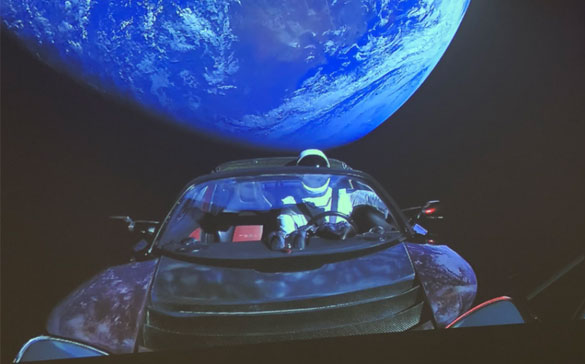
\includegraphics[width=0.5\textwidth]{tesla.jpg}
%\caption{\label{fig:tesla}Esta imagen se añadió en el menú Project.}
%\end{figure}


\subsection{The Newmark's method without damping}


If we start at the beginning, the equation for the elastodynamics model means

\begin{align}
\rho \frac{\partial^2 u}{\partial t^2} & = E  \frac{\partial^2 u}{\partial x^2} \text{ in } (0,L) \times (0,T) \label{e1}\\
u(0,t) & = u^0(t) \text{ in } (0,T) \label{e2}\\
u(L,t) & = u^{N_x}(t)  \text{ in } (0,T) \label{e3} \\
u(x,0) & = u_0(x)  \text{ in } (0,L) \label{e4}\\
\dot{u}(x,0) &  = v_0(x)  \text{ in } (0,T) \label{e5}
\end{align}
Take $i\Delta x = i L/N_x = x_i$ and $u^{i}(t):=u(x_i,t)$  for $0 \le i \le N_x.$ Then \eqref{e1} means
\begin{align}
\frac{\rho}{E} \frac{\partial^2 u^i}{\partial t^2}  = \frac{1}{2\Delta x^2} \left(u^{i+1}(t) -2u^i(t)+u^{i-1}(t)\right),
\end{align}
that is
\begin{align}
\frac{\rho}{E} \ddot{u}^i(t)  = \frac{1}{2\Delta x^2} \left(u^{i+1}(t) -2u^i(t)+u^{i-1}(t)\right), \label{1eq1}
\end{align}
for $1 \le i \le N_x-1.$ Take
$$
\mathbf{u}(t):=(u^1(t),\ldots,u^{N_x-1}(t))^T \in \mathbb{R}^{N_x-1}
$$
and write \eqref{1eq1} as
\begin{align}
M \ddot{\mathbf{u}}(t)  + K \mathbf{u}(t) = \mathbf{F}(t) \label{Peq}
\end{align}
where $M = \frac{\rho}{E} \, id_{(N_x-1) \times (N_x-1)},$ 
$$
K = \left[
\begin{array}{ccccccc}
-2 & 1 & 0 & \cdots & 0 & 0 & 0 \\
1 & -2 & 1 & \cdots & 0 & 0 & 0 \\
0 & 1 & -2 & \cdots & 0 & 0 & 0 \\
\vdots & \vdots & \vdots & \ddots & \vdots & \vdots & \vdots \\
0 & 0 & 0 & \cdots & 1 & -2 & 1 \\
0 & 0 & 0 & \cdots & 0 & 1 & -2
\end{array}
\right]_{(N_x-1) \times (N_x-1)}
$$
is the matrix of discrete Laplacian and, finally,
$$
\mathbf{F}(t) = -\frac{1}{2\Delta x^2}\,(u^0(t),0,\ldots,0,u^{N_x}(t))^T.
$$
Now, consider $t_i = i \,\Delta t = i \, T/N_t$ and 
$$
\mathbf{u}(t_i) = (u^1(t_i),\ldots,u^{N_x-1}(t_i))^T = (u^1_i,\ldots,u^{N_x-1}_i) \in \mathbb{R}^{N_x-1}
$$
for $0 \le i \le N_t.$ We known
$$
\mathbf{u}(t_0) = (u(x_1,0),\ldots,u(x_{N_x-1},0))^T = (u_0(x_1),\ldots,u_0(x_{N_x-1}))^T.
$$
%%%%%%%  PAGINA 1

and

$$
\dot{\mathbf{u}}(t_0) = (\dot{u}(x_1,0),\ldots,\dot{u}(x_{N_x-1},0))^T = (v_0(x_1),\ldots,v_0(x_{N_x-1}))^T.
$$

%%%%% Newmark
Then the Newmark's method reads 
\begin{align}
\dot{\mathbf{u}}(t_i) &z = \dot{\mathbf{u}}(t_{i-1}) + \Delta t (1-\gamma) \ddot{\mathbf{u}}(t_{i-1}) + \Delta t \gamma  \ddot{\mathbf{u}}(t_{i}) \label{N1}\\
\mathbf{u}(t_i) & = \mathbf{u}(t_{i-1})+\Delta t  \dot{\mathbf{u}(t_{i-1})}
+(1-2\beta)\frac{\Delta t^2}{2} \ddot{\mathbf{u}(t_{i-1})}+\beta \Delta t^2  \ddot{\mathbf{u}(t_{i})} \label{N2}
\end{align}
Rearranging \eqref{N2} to provide an expression for $ \ddot{\mathbf{u}}(t_{i})$ that dividing by $\beta \Delta t^2$ gives us
\begin{align}
\ddot{\mathbf{u}}(t_{i}) = \frac{\mathbf{u}(t_{i})-\mathbf{u}(t_{i-1})}{\beta \Delta t^2} - \frac{1}{\beta \Delta t} \dot{\mathbf{u}}(t_{i-1})
-\left( \frac{1}{2\beta}-1\right)\ddot{\mathbf{u}}(t_{i-1}), \label{ddot1}
\end{align}
and, inserting the expression for $\ddot{\mathbf{u}}(t_{i})$ from above into \eqref{N1} gives:
\begin{align}
\dot{\mathbf{u}}(t_{i}) = \frac{\gamma(\mathbf{u}(t_{i})-\mathbf{u}(t_{i-1}))}{\beta \Delta t} + \left( 1 - \frac{\gamma}{\beta }\right)  \dot{\mathbf{u}}(t_{i-1})
+\Delta t \left( 1-\frac{\gamma}{2\beta}\right)\ddot{\mathbf{u}}(t_{i-1}) \label{dot1}
\end{align}
We insert the explicit expression of \eqref{N2} into \eqref{Peq} to obtain
\begin{align}
 M \ddot{\mathbf{u}}(t_{i})  + K \left(\mathbf{u}(t_{i-1}) + \Delta t \dot{\mathbf{u}}(t_{i-1})
- \Delta t^2 \left( \beta -\frac{1}{2}\right)\ddot{\mathbf{u}}(t_{i-1}) + \Delta t^2 \beta \ddot{\mathbf{u}}(t_{i}) \right)   = \mathbf{F}(t_{i})\label{newmark}
\end{align}
and where
$$
\ddot{\mathbf{u}}(t_0) = M^{-1}\left( \mathbf{F}(t_0) - K \mathbf{u}(t_0) \right).
$$
Now, put
\begin{align*}
\mathbf{U} & = \left[\mathbf{u}(t_1) \mathbf{u}(t_2) \cdots \mathbf{u}(t_{N_t})\right] \in \mathbb{R}^{(N_x-1) \times N_t} \\
\dot{\mathbf{U}} & = \left[\dot{\mathbf{u}}(t_1) \dot{\mathbf{u}}(t_2) \cdots \dot{\mathbf{u}}(t_{N_t})\right] \in \mathbb{R}^{(N_x-1) \times N_t} \\
\ddot{\mathbf{U}} & = \left[\ddot{\mathbf{u}}(t_1) \ddot{\mathbf{u}}(t_2) \cdots \ddot{\mathbf{u}}(t_{N_t})\right] \in \mathbb{R}^{(N_x-1) \times N_t} 
\end{align*}
and define
$$
\mathrm{vec}(\mathbf{U}) = \left[
\begin{array}{c}
\mathbf{u}(t_1)\\
\mathbf{u}(t_2) \\
\vdots \\
\mathbf{u}(t_{N_t}) 
\end{array}
\right] \in \mathbb{R}^{N_t(N_x-1)}.
$$
Then we can write \eqref{newmark}  as
\begin{align*}
\left[
\begin{array}{ccccccc}
\Delta t^2 \beta K + M & 0 & 0  &\cdots & 0 & 0 & 0 \\
\Delta t^2 \left( \frac{1}{2} - \beta \right) K & \Delta t^2 \beta K + M & 0 & \cdots & 0 & 0 & 0 \\
0 & \Delta t^2 \left( \frac{1}{2} - \beta \right) K & \Delta t^2 \beta K + M & \cdots & 0 & 0 & 0 \\
\vdots & \vdots & \vdots & \ddots & \vdots & \vdots & \vdots \\
0 & 0 & 0 & \cdots & \Delta t^2 \left( \frac{1}{2} - \beta \right) K & \Delta t^2 \beta K + M & 0 \\
0 & 0 & 0 & \cdots & 0 & \Delta t^2 \left( \frac{1}{2} - \beta \right) K  & \Delta t^2 \beta K + M \\
\end{array}
\right]\left[
\begin{array}{c}
\ddot{\mathbf{u}}(t_1)\\
\ddot{\mathbf{u}}(t_2) \\
\vdots \\
\ddot{\mathbf{u}}(t_{N_t}) 
\end{array}
\right] +  \\
\Delta t \left[
\begin{array}{ccccccc}
0 & 0 & 0  &\cdots & 0 & 0 & 0 \\
 K & 0 & 0 & \cdots & 0 & 0 & 0 \\
0 & K & 0 & \cdots & 0 & 0 & 0 \\
\vdots & \vdots & \vdots & \ddots & \vdots & \vdots & \vdots \\
0 & 0 & 0 & \cdots & K & 0 & 0 \\
0 & 0 & 0 & \cdots & 0 & K  & 0 \\
\end{array}
\right]\left[
\begin{array}{c}
\dot{\mathbf{u}}(t_1)\\
\dot{\mathbf{u}}(t_2) \\
\vdots \\
\dot{\mathbf{u}}(t_{N_t}) 
\end{array}
\right] + \\
\left[
\begin{array}{ccccccc}
0 & 0 & 0  &\cdots & 0 & 0 & 0 \\
 K & 0 & 0 & \cdots & 0 & 0 & 0 \\
0 & K & 0 & \cdots & 0 & 0 & 0 \\
\vdots & \vdots & \vdots & \ddots & \vdots & \vdots & \vdots \\
0 & 0 & 0 & \cdots & K & 0 & 0 \\
0 & 0 & 0 & \cdots & 0 & K  & 0 \\
\end{array}
\right]\left[
\begin{array}{c}
\mathbf{u}(t_1)\\
\mathbf{u}(t_2) \\
\vdots \\
\mathbf{u}(t_{N_t}) 
\end{array}
\right] =
\left[
\begin{array}{c}
\mathbf{F}(t_1)\\
\mathbf{F}(t_2) \\
\vdots \\
\mathbf{F}(t_{N_t}) 
\end{array}
\right] + 
\left[
\begin{array}{c}
-  K  \mathbf{u}(t_0) - \Delta t K \dot{\mathbf{u}}(t_0) - \Delta t^2 \left( \frac{1}{2}-\beta \right) K \ddot{\mathbf{u}}(t_0)\\
\mathbf{0} \\
\vdots \\
\mathbf{0} 
\end{array}
\right],
\end{align*}

%%%%%%%%%% PAGINA 2


that is
\begin{align}
\begin{array}{c}
\left(D_0 \otimes K + id_{N_t \times N_t} \otimes  M  \right) \mathrm{vec}(\ddot{\mathbf{U}}) - \Delta t \left(D_4 \otimes  \frac{M}{\beta\, \Delta t^2}\right)\mathrm{vec}(\dot{\mathbf{U}}) \\
- \left( D_4 \otimes   K\right)\mathrm{vec}(\mathbf{U}) =
\mathbf{a},
\end{array}\label{newmark1}
\end{align}
where
$$
D_0 := \left[
\begin{array}{cccccc}
\Delta t^2 \beta  & 0 & 0 & \cdots & 0 & 0 \\
\Delta t^2 \left(\frac{1}{2} - \beta \right) & \Delta t^2 \beta & 0 & \cdots & 0 & 0 \\
0 & \Delta t^2 \left(\frac{1}{2} - \beta \right) & \Delta t^2 \beta & \cdots & 0 & 0 \\
\vdots & \vdots & \vdots & \ddots & \vdots & \vdots \\
0 & 0 & 0 & \cdots & \Delta t^2 \beta & 0 \\
0 & 0 & 0 & \cdots & \Delta t^2 \left(\frac{1}{2} - \beta \right) & \Delta t^2 \beta  
\end{array}  
\right],
$$
$$
D_4 := \left[
\begin{array}{cccccc}
0  & 0 & 0 & \cdots & 0 & 0 \\
-1 & 0 & 0 & \cdots & 0 & 0 \\
0 & -1 & 0 & \cdots & 0 & 0 \\
\vdots & \vdots & \vdots & \ddots & \vdots & \vdots \\
0 & 0 & 0 & \cdots & 0 & 0 \\
0 & 0 & 0 & \cdots & -1 & 0 
\end{array}  
\right],
$$
$$
\mathbf{a}:= \left[
\begin{array}{c}
\mathbf{F}(t_1)\\
\mathbf{F}(t_2) \\
\vdots \\
\mathbf{F}(t_{N_t}) 
\end{array}
\right] + 
\left[
\begin{array}{c}
-  K  \mathbf{u}(t_0) - \Delta t K \dot{\mathbf{u}}(t_0) - \Delta t^2 \left( \frac{1}{2}-\beta \right) K \ddot{\mathbf{u}}(t_0)\\
\mathbf{0} \\
\vdots \\
\mathbf{0} 
\end{array}
\right].
$$


Proceeding in a similar way with \eqref{N1} and \eqref{N2} we obtain
\begin{align*}
\left[
\begin{array}{ccccccc}
id_{(N_x-1)\times(N_x-1)}& 0 & 0  &\cdots & 0 & 0 \\
 -id_{(N_x-1)\times(N_x-1)} & id_{(N_x-1)\times(N_x-1)} & 0 & \cdots & 0 & 0 \\
0 & -id_{(N_x-1)\times(N_x-1)} & id_{(N_x-1)\times(N_x-1)} & \cdots & 0 & 0 \\
\vdots & \vdots & \vdots & \ddots & \vdots & \vdots \\
0 & 0 & 0 & \cdots & id_{(N_x-1)\times(N_x-1)}  & 0 \\
0 & 0 & 0 & \cdots & -id_{(N_x-1)\times(N_x-1)} &  id_{(N_x-1)\times(N_x-1)} \\
\end{array}
\right]\left[
\begin{array}{c}
\dot{\mathbf{u}}(t_1)\\
\dot{\mathbf{u}}(t_2) \\
\vdots \\
\dot{\mathbf{u}}(t_{N_t}) 
\end{array}
\right] -
\end{align*}
\begin{align*}
\Delta t\left[
\begin{array}{cccccc}
 \gamma id_{(N_x-1)\times(N_x-1)} & 0 & 0  &\cdots & 0 & 0 \\
 \left(1-\gamma\right)id_{(N_x-1)\times(N_x-1)} & \gamma id_{(N_x-1)\times(N_x-1)} & 0 &  \cdots & 0 & 0  \\
\vdots & \vdots & \vdots & \ddots & \vdots & \vdots  \\
0 & 0 & 0 &\cdots & \left(1-\gamma\right)id_{(N_x-1)\times(N_x-1)} & \gamma id_{(N_x-1)\times(N_x-1)}
\end{array}
\right]\left[
\begin{array}{c}
\ddot{\mathbf{u}}(t_1)\\
\ddot{\mathbf{u}}(t_2) \\
\vdots \\
\ddot{\mathbf{u}}(t_{N_t}) 
\end{array}
\right] = \\
\left[
\begin{array}{c}
\dot{\mathbf{u}}(t_0) + \left(1-\gamma\right)\Delta t\ddot{\mathbf{u}}(t_0) \\
\mathbf{0} \\
\vdots \\
\mathbf{0} 
\end{array}
\right],
\end{align*}


%%%%%%%%%% PAGINA 3



Introduce the following two matrices
$$
D_1 = \left[
\begin{array}{cccccc}
1 & 0 & 0 & \cdots & 0 & 0 \\
-1 & 1 & 0 & \cdots & 0 & 0 \\
0 & -1 & 1 & \cdots & 0 & 0 \\
\vdots & \vdots & \vdots & \ddots & \vdots & \vdots \\
0 & 0 & 0 & \cdots & 1 & 0 \\
0 & 0 & 0 & \cdots & -1 & 1  
\end{array}  
\right]
\text{ and } 
D_2 = \left[
\begin{array}{cccccc}
\gamma & 0 & 0 & \cdots & 0 & 0 \\
\left( 1-\gamma \right) & \gamma & 0 & \cdots & 0 & 0 \\
0 & \left( 1-\gamma\right) & 1 & \cdots & 0 & 0 \\
\vdots & \vdots & \vdots & \ddots & \vdots & \vdots \\
0 & 0 & 0 & \cdots & \gamma & 0 \\
0 & 0 & 0 & \cdots & \left(1-\gamma\right) & \gamma 
\end{array}  
\right].
$$
Observe that 
$$
D_1^{-1} = \left[
\begin{array}{cccccc}
1 & 0 & 0 & \cdots & 0 & 0 \\
1 & 1 & 0 & \cdots & 0 & 0 \\
1 & 1 & 1 & \cdots & 0 & 0 \\
\vdots & \vdots & \vdots & \ddots & \vdots & \vdots \\
1 & 1 & 1 & \cdots & 1 & 0 \\
1 & 1 & 1 & \cdots & 1 & 1  
\end{array}  
\right].
$$
Then \eqref{ddot1} can be written as
\begin{align}
\begin{array}{c}
\left( D_1 \otimes  id_{(N_x-1)\times(N_x-1)}\right) \mathrm{vec}(\dot{\mathbf{U}}) - \Delta t \left( D_2 \otimes  id_{(N_x-1)\times(N_x-1)}\right) \mathrm{vec}(\ddot{\mathbf{U}}) = \mathbf{b}
\end{array}\label{newmark2}
\end{align}
where
$$
\mathbf{b}:= \left[
\begin{array}{c}
\dot{\mathbf{u}}(t_0) + \left(1-\gamma\right)\Delta t\ddot{\mathbf{u}}(t_0) \\
\mathbf{0} \\
\vdots \\
\mathbf{0} 
\end{array}
\right].
$$
Thus,
$$
\mathrm{vec}(\dot{\mathbf{U}}) = \left( D_1^{-1} \otimes  id_{(N_x-1)\times(N_x-1)}\right)\left( \mathbf{b} +  \Delta t \left( D_2 \otimes  id_{(N_x-1)\times(N_x-1)}\right) \mathrm{vec}(\ddot{\mathbf{U}})\right)
$$

Finally, we can compute \eqref{N2} following the same strategy to obtain by using the matrix
$$
D_3 = \left[
\begin{array}{cccccc}
\beta & 0 & 0 & \cdots & 0 & 0 \\
\frac{1}{2}-\beta  & \beta & 0 & \cdots & 0 & 0 \\
0 &\frac{1}{2}-\beta  & \beta & \cdots & 0 & 0 \\
\vdots & \vdots & \vdots & \ddots & \vdots & \vdots \\
0 & 0 & 0 & \cdots & \beta & 0 \\
0 & 0 & 0 & \cdots &\frac{1}{2}-\beta & \beta 
\end{array}  
\right].
$$
We obtain
\begin{align}
\begin{array}{c}
\left( D_1 \otimes  id_{(N_x-1)\times(N_x-1)}\right) \mathrm{vec}(\mathbf{U}) + \Delta t
\left(D_4 \otimes  id_{(N_x-1)\times(N_x-1)} \right)\mathrm{vec}(\dot{\mathbf{U}}) \\ - \Delta t^2 \left( D_3 \otimes  id_{(N_x-1)\times(N_x-1)} \right) \mathrm{vec}(\ddot{\mathbf{U}}) = \mathbf{c}
\end{array}\label{newmark3}
\end{align}\
where
$$
\mathbf{c}:= \left[
\begin{array}{c}
\mathbf{u}(t_0) + \Delta t \, \dot{\mathbf{u}}(t_0) + \Delta t^2 \left(\frac{1}{2}-\beta\right)\ddot{\mathbf{u}}(t_0)+  \\
\mathbf{0} \\
\vdots \\
\mathbf{0} 
\end{array}
\right].
$$


We remark that
\begin{align*}
\mathrm{vec}(\mathbf{U}) =\left( D_1^{-1} \otimes  id_{(N_x-1)\times(N_x-1)}\right) \times \\
\left( \mathbf{c} - 
\Delta t
\left(D_4 \otimes  id_{(N_x-1)\times(N_x-1)} \right)\mathrm{vec}(\dot{\mathbf{U}}) + \Delta t^2 \left( D_3 \otimes  id_{(N_x-1)\times(N_x-1)} \right) \mathrm{vec}(\ddot{\mathbf{U}})
\right) 
\end{align*}
where
$$
\mathrm{vec}(\dot{\mathbf{U}}) = \left( D_1^{-1} \otimes  id_{(N_x-1)\times(N_x-1)}\right)\left( \mathbf{b} +  \Delta t \left( D_2 \otimes  id_{(N_x-1)\times(N_x-1)}\right) \mathrm{vec}(\ddot{\mathbf{U}})\right).
$$
By substituting both in \eqref{newmark1} we obtain:
$$
\begin{array}{c}
\left(D_0 \otimes K + id_{N_t \times N_t} \otimes  M  \right) \mathrm{vec}(\ddot{\mathbf{U}}) - \Delta t \left(D_4 \otimes  K \right) \\
\times \left( D_1^{-1} \otimes  id_{(N_x-1)\times(N_x-1)}\right) \times \left( \mathbf{b} +  \Delta t \left( D_2 \otimes  id_{(N_x-1)\times(N_x-1)}\right) \mathrm{vec}(\ddot{\mathbf{U}})\right) \\ 
 -  \left( D_4 \otimes   K\right) \times \left( D_1^{-1} \otimes  id_{(N_x-1)\times(N_x-1)}\right) \\ 
\times \left( \mathbf{c} - \Delta t \left(D_4 \otimes  id_{(N_x-1)\times(N_x-1)} \right) \times \left( D_1^{-1} \otimes  id_{(N_x-1)\times(N_x-1)}\right) \right. \\
\left. \times \left( \mathbf{b} +  \Delta t \left( D_2 \otimes  id_{(N_x-1)\times(N_x-1)}\right) \mathrm{vec}(\ddot{\mathbf{U}})\right) + \Delta t^2 \left( D_3 \otimes  id_{(N_x-1)\times(N_x-1)} \right) \mathrm{vec}(\ddot{\mathbf{U}}) \right)   =
\mathbf{a},
\end{array}
$$

that is a linear equation in $\mathrm{vec}(\ddot{\mathbf{U}}).$ So we can get $\mathrm{vec}(\ddot{\mathbf{U}})$ as follows:

$$
\begin{array}{c}
\mathrm{vec}(\ddot{\mathbf{U}}) = \left(\left(D_0 \otimes K + id_{N_t \times N_t} \otimes  M  \right) - \Delta t \left(D_4 \otimes  K \right) \times \left( D_1^{-1} \otimes  id_{(N_x-1)\times(N_x-1)}\right)   \right.\\
\left. \Delta t \left( D_2 \otimes  id_{(N_x-1)\times(N_x-1)}\right) -  \left( D_4 \otimes   K\right) \times \left( D_1^{-1} \otimes  id_{(N_x-1)\times(N_x-1)}\right) \right. \\
\left.  \times \left( - \Delta t \left(D_4 \otimes  id_{(N_x-1)\times(N_x-1)} \right) \times \left( D_1^{-1} \otimes  id_{(N_x-1)\times(N_x-1)}\right) \right. \right. \\
\left. \left. \Delta t \left( D_2 \otimes  id_{(N_x-1)\times(N_x-1)}\right)  + \Delta t^2 \left( D_3 \otimes  id_{(N_x-1)\times(N_x-1)} \right) \right) \right)^{-1} \\
\times \left( \Delta t \left(D_4 \otimes  K \right) \times \left( D_1^{-1} \otimes  id_{(N_x-1)\times(N_x-1)}\right)  \mathbf{b} +\left( D_4 \otimes   K\right) \times \left( D_1^{-1} \otimes  id_{(N_x-1)\times(N_x-1)}\right) \right. \\
\left.  \times \left( - \Delta t \left(D_4 \otimes  id_{(N_x-1)\times(N_x-1)} \right) \times \left( D_1^{-1} \otimes  id_{(N_x-1)\times(N_x-1)}\right) \mathbf{b}  + \mathbf{c}  \right) + \mathbf{a}  \right), \\
\end{array}
$$





\subsection{The Newmark's method with damping}


As has been done in the previous section, we can write \eqref{1eq1} including damping as follows
\begin{align}
M \ddot{\mathbf{u}}(t) + C \dot{\mathbf{u}}(t)  + K \mathbf{u}(t) = \mathbf{F}(t) \label{PeqC}
\end{align}
We insert the explicit expression of \eqref{N2} into \eqref{PeqC} to obtain
\begin{align}
 M \ddot{\mathbf{u}}(t_{i})  + C \left(\dot{\mathbf{u}}(t_{i-1})
- \Delta t \left( \gamma -1\right)\ddot{\mathbf{u}}(t_{i-1}) + \Delta t \gamma \ddot{\mathbf{u}}(t_{i}) \right) \\
+ K \left(\mathbf{u}(t_{i-1}) + \Delta t \dot{\mathbf{u}}(t_{i-1})
- \Delta t^2 \left( \beta -\frac{1}{2}\right)\ddot{\mathbf{u}}(t_{i-1}) + \Delta t^2 \beta \ddot{\mathbf{u}}(t_{i}) \right)   = \mathbf{F}(t_{i})\label{newmarkC}
\end{align}
and where
$$
\ddot{\mathbf{u}}(t_0) = M^{-1}\left( \mathbf{F}(t_0) - C \dot{\mathbf{u}}(t_0) - K \mathbf{u}(t_0) \right).
$$
Then we can write \ref{newmarkC} as
\begin{align}
\begin{array}{c}
\left(D_0 \otimes K + \Delta t D_2 \otimes C + id_{N_t \times N_t} \otimes  M  \right) \mathrm{vec}(\ddot{\mathbf{U}}) - \left(D_4 \otimes  \left(C+\Delta t K\right)\right)\mathrm{vec}(\dot{\mathbf{U}}) \\
- \left( D_4 \otimes   K\right)\mathrm{vec}(\mathbf{U}) =
\mathbf{a},
\end{array}\label{newmark13}
\end{align}
There is only a vector that changes from previous section being now
$$
\mathbf{a}:= \left[
\begin{array}{c}
\mathbf{F}(t_1)\\
\mathbf{F}(t_2) \\
\vdots \\
\mathbf{F}(t_{N_t}) 
\end{array}
\right] + 
\left[
\begin{array}{c}
-  K  \mathbf{u}(t_0) - \left( C + \Delta t K \right) \dot{\mathbf{u}}(t_0) - \left( \Delta t \left(1 - \gamma \right) C + \Delta t^2 \left( \frac{1}{2}-\beta \right) K \right)\ddot{\mathbf{u}}(t_0)\\
\mathbf{0} \\
\vdots \\
\mathbf{0} 
\end{array}
\right].
$$
Proceeding in the same way as past section we can get $\mathrm{vec}(\ddot{\mathbf{U}})$ as follows:
$$
\begin{array}{c}
\mathrm{vec}(\ddot{\mathbf{U}}) = \left(\left(D_0 \otimes K + \Delta t D_2 \otimes C + id_{N_t \times N_t} \otimes  M  \right) - \left(D_4 \otimes  \left(C+\Delta t K\right)\right) \times \left( D_1^{-1} \otimes  id_{(N_x-1)\times(N_x-1)}\right)   \right.\\
\left. \Delta t \left( D_2 \otimes  id_{(N_x-1)\times(N_x-1)}\right) -  \left( D_4 \otimes   K \right) \times \left( D_1^{-1} \otimes  id_{(N_x-1)\times(N_x-1)}\right) \right. \\
\left.  \times \left( - \Delta t \left(D_4 \otimes  id_{(N_x-1)\times(N_x-1)} \right) \times \left( D_1^{-1} \otimes  id_{(N_x-1)\times(N_x-1)}\right) \right. \right. \\
\left. \left. \Delta t \left( D_2 \otimes  id_{(N_x-1)\times(N_x-1)}\right)  + \Delta t^2 \left( D_3 \otimes  id_{(N_x-1)\times(N_x-1)} \right) \right) \right)^{-1} \\
\times \left( \left(D_4 \otimes  \left( C + \Delta t K\right) \right) \times \left( D_1^{-1} \otimes  id_{(N_x-1)\times(N_x-1)}\right)  \mathbf{b} +\left( D_4 \otimes   K\right) \times \left( D_1^{-1} \otimes  id_{(N_x-1)\times(N_x-1)}\right) \right. \\
\left.  \times \left( - \Delta t \left(D_4 \otimes  id_{(N_x-1)\times(N_x-1)} \right) \times \left( D_1^{-1} \otimes  id_{(N_x-1)\times(N_x-1)}\right) \mathbf{b}  + \mathbf{c}  \right) + \mathbf{a}  \right), \\
\end{array}
$$




\subsection{Greedy Rank-One Update Algorithm}

The most important part of the simulator deals with the Greedy Rank-One Update Algorithm (or as it has been called GROUA in previous sections). In this section we will try to explain how this method works, as well as the main equations that form it.

The method consists of iteratively evaluating a for loop, which extracts a remainder and the acceleration vector as outputs. If this residual is less than a stipulated error, the acceleration vector is correct. If, on the other hand, this remainder is greater than this error, the for loop is executed again. This is reflected in the figure \ref{Main loop}, which is a block diagram that summarizes the operation of the method. As input to the program, the matrix system obtained in the previous section is given, which had been obtained after developing the Newmark equations in a tensorial form.


For the case without damping, the input elements are:

$$
\begin{array}{c}
A = \left(D_0 \otimes K + id_{N_t \times N_t} \otimes  M  \right) - \Delta t \left(D_4 \otimes  K \right) \times \left( D_1^{-1} \otimes  id_{(N_x-1)\times(N_x-1)}\right)  \\
\left. \Delta t \left( D_2 \otimes  id_{(N_x-1)\times(N_x-1)}\right) -  \left( D_4 \otimes   K\right) \times \left( D_1^{-1} \otimes  id_{(N_x-1)\times(N_x-1)}\right) \right. \\
\left.  \times \left( - \Delta t \left(D_4 \otimes  id_{(N_x-1)\times(N_x-1)} \right) \times \left( D_1^{-1} \otimes  id_{(N_x-1)\times(N_x-1)}\right) \right. \right.\\
\left. \Delta t \left( D_2 \otimes  id_{(N_x-1)\times(N_x-1)}\right)  + \Delta t^2 \left( D_3 \otimes  id_{(N_x-1)\times(N_x-1)} \right) \right)
\end{array}
$$

$$
\begin{array}{c}
b = \Delta t \left(D_4 \otimes  K \right) \times \left( D_1^{-1} \otimes  id_{(N_x-1)\times(N_x-1)}\right)  \mathbf{b} +\left( D_4 \otimes   K\right) \times \left( D_1^{-1} \otimes  id_{(N_x-1)\times(N_x-1)}\right) \\
 \times \left( - \Delta t \left(D_4 \otimes  id_{(N_x-1)\times(N_x-1)} \right) \times \left( D_1^{-1} \otimes  id_{(N_x-1)\times(N_x-1)}\right) \mathbf{b}  + \mathbf{c}  \right) + \mathbf{a} \\
\end{array}
$$



While for the case with damping the input elements are:

$$
\begin{array}{c}
A = \left(D_0 \otimes K + \Delta t D_2 \otimes C + id_{N_t \times N_t} \otimes  M  \right) - \left(D_4 \otimes  \left(C+\Delta t K\right)\right) \times \left( D_1^{-1} \otimes  id_{(N_x-1)\times(N_x-1)}\right) \\
\left. \Delta t \left( D_2 \otimes  id_{(N_x-1)\times(N_x-1)}\right) -  \left( D_4 \otimes   K \right) \times \left( D_1^{-1} \otimes  id_{(N_x-1)\times(N_x-1)}\right) \right. \\
\left.  \times \left( - \Delta t \left(D_4 \otimes  id_{(N_x-1)\times(N_x-1)} \right) \times \left( D_1^{-1} \otimes  id_{(N_x-1)\times(N_x-1)}\right) \right. \right. \\
 \left. \Delta t \left( D_2 \otimes  id_{(N_x-1)\times(N_x-1)}\right)  + \Delta t^2 \left( D_3 \otimes  id_{(N_x-1)\times(N_x-1)} \right) \right)  \\
\end{array}
$$

$$
\begin{array}{c}
b = \left(D_4 \otimes  \left( C + \Delta t K\right) \right) \times \left( D_1^{-1} \otimes  id_{(N_x-1)\times(N_x-1)}\right)  \mathbf{b} +\left( D_4 \otimes   K\right) \times \left( D_1^{-1} \otimes  id_{(N_x-1)\times(N_x-1)}\right)  \\
  \times \left( - \Delta t \left(D_4 \otimes  id_{(N_x-1)\times(N_x-1)} \right) \times \left( D_1^{-1} \otimes  id_{(N_x-1)\times(N_x-1)}\right) \mathbf{b}  + \mathbf{c}  \right) + \mathbf{a} \\
\end{array}
$$



\begin{figure}
\centering
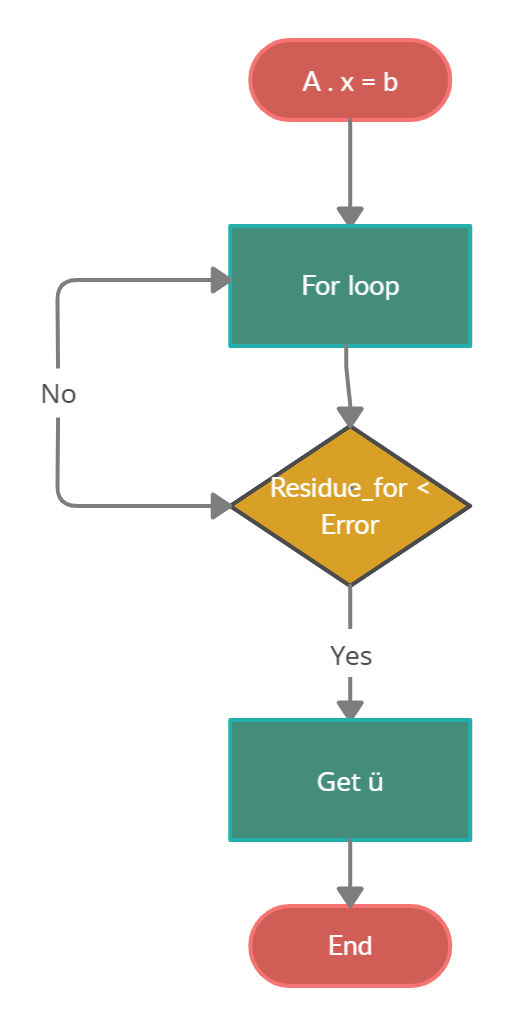
\includegraphics[width=0.30\textwidth]{Main block (1).png}
\caption{Main loop} 
\label{Main loop}
\end{figure}


If the for loop itself is analyzed, as can be seen in the figure\ref{For loop}, its structure is very similar to the structure of the general method. As before, a loop is also iteratively evaluated, in this case called while. As with the main loop, if the extracted residue is less than a tolerance, the necessary outputs are obtained for the evaluation of the upper loop (for loop). If not, the while loop is executed again. Unlike what happened in the other loop, each time the for loop is entered, initial conditions are generated, which are random.


\begin{figure}
\centering
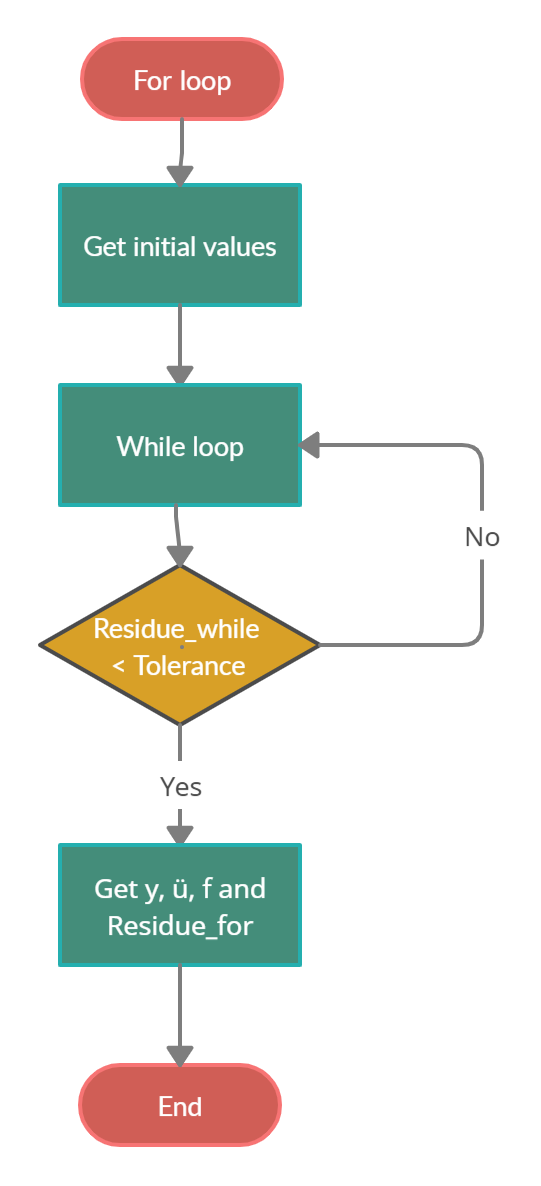
\includegraphics[width=0.30\textwidth]{For loop (1).png}
\caption{For loop} 
\label{For loop}
\end{figure}

The equations found in the while loop and how to proceed are as follows: First the previous value of the vector $x_10$ is saved, which in the first iteration is random.
\begin{equation}
    x_{1} = x_{10}
\end{equation}
After this, the matrix $Z_1$ is generated and the new value of $x_{10}$ is calculated.
\begin{equation}
    Z_1 = A I_t \otimes  x_{20}
\end{equation}
\begin{equation}
    x_{10} = Z_1^{-1} f
\end{equation}
Once the new $x_{10}$ is obtained, the tolerance between this vector and the previously saved one is calculated.
\begin{equation}
    tol_1 = |x_{10}-x_1|
\end{equation}
It proceeds in the same way for all the present state vectors, taking as tolerance the one with the highest absolute value of all of them. The loop will end when said tolerance is less than the one imposed as allowed. After finishing with the while loop, the value of $y$ is updated, being this:
\begin{equation}
    y = x_{10} \otimes  x_{20}
\end{equation}
The accumulation of the different values of $y$ is what will ultimately give the acceleration vector $\ddot{u}$. Although for this it is necessary to carry out several iterations repeating the process, therefore, the variable $fn$ is created, which indicates how close $y$ is to being correct.
\begin{equation}
    fn = f - A y
\end{equation}
From the residue of $fn$, the residue of the for loop itself is obtained in the same way as the previous ones, which must be less than the previously imposed value in order to consider the calculation finished. Until this happens, the value of $fn$ is saved as the next $f$ and starts over.

Once the correct $\ddot{u}$ has been obtained and with what has been explained in the previous points, it is straightforward to obtain $\dot{u}$ and $u$.

%%% Ecuaciones del while




%%%%%%%%%%%%%%%%%%%%%%%%%%%%%%%%%%%%%%%%
%%%%%% SECCIÓN 4 %%%%%%%%%%%%%%%%%%%%%%%
%%%%%%%%%%%%%%%%%%%%%%%%%%%%%%%%%%%%%%%%


\section{About the convergence and stability of the tensor-based Newmark's method}

This section will comment on the stability and convergence studies and their respective results, if any. This study is of utmost importance, mainly because if the method is not stable, it could give inconsistent results or not provide a solution, and if the results are not converged, the results would be erroneous.

%% Estabilidad, referencia de los japos %%

To carry out the study of the stability of the method, it is necessary to differentiate between two cases: for $\frac{1}{2} \gamma \leq \beta$ and for $0 \leq \beta < \frac{1}{2} \ gamma$. Despite having been programmed for both cases, for the study carried out only one of them will be emphasized, since $\beta = \frac{1}{6} < \frac{1}{2} \gamma$.
For this specific case there is a condition that the time step must meet for the method to be stable: $\tau < \sqrt{\frac{1}{(\frac{1}{2} \gamma - \beta) || K^{1/2}||^2}} $.
Therefore, the method is stable as long as the following condition  is fulfilled:
\begin{equation}
    \|\mathbf{u}(t)\| \leq \|\mathbf{u}(0)\| + \sqrt{\frac{C_0}{1-\tau^2 (\frac{1}{2} \gamma - \beta) \|K^{1/2}\|^2}t}
\end{equation}
being:
\begin{equation}
    C_0 = \|\dot{\mathbf{u}}(0)\|^2 + \tau^2 (\beta - \frac{1}{2} \gamma + \frac{1}{4}) \|K^{1/2} \dot{\mathbf{u}}(0) \|^2 + \tau (K \dot{\mathbf{u}}(0) \cdot \mathbf{u}(0)) + \| K^{1/2} \mathbf{u}(0) \|^2 + \tau (\gamma - \frac{1}{2}) \| C^{1/2} \dot{\mathbf{u}}(0) \|^2
\end{equation}
For each executed case, the values change, but the condition of the upper equation must always be met to ensure stability. Stability values will be included in the examples to be described later.\\

%% Convergencia, sobre todo convergencia numérica %%

Regarding convergence, knowing that Newmark's method converges adequately, and also that GROUA itself converges numerically, it can be said that the simulator in general converges. This can be seen more clearly in the evolution of the residual as the iterations increase. The figure \ref{ResIter} shows this evolution, making it clear that from iteration 2, the solution has converged because of the value of que residue. %Furthermore, in the same figure the limit that marks the maximum permissible error has been included, allowing the correct convergence of the method to be concluded at a glance. Keep in mind that the value selected for the error is very small, on the order of (-8).

In order to better observe the trend, the first residual has been eliminated from the graph, which is very large due to the randomness of the code initially. Furthermore, it has been deemed convenient not to include the value selected for the error ($ 10{-8}$), as happens later.

In order to better observe the trend of the residue, the figure \ref{ResIterLog} has been included, which has the residue on a logarithmic scale. Despite the downward trend, the solution does not improve after iteration 2, although for safety we will say that after iteration 5 the solution has converged. In addition, in this figure the maximum allowed error has been included, in order to make it clear that it is exceeded in the first iterations.

\begin{figure}
\centering
\includegraphics[width=0.75\textwidth]{ResIter.eps}
\caption{Residue evolution vs Iterations } 
\label{ResIter}
\end{figure}

\begin{figure}
\centering
\includegraphics[width=0.75\textwidth]{ResIterLog.eps}
\caption{Residue evolution (Log scale) vs Iterations } 
\label{ResIterLog}
\end{figure}

%%%%%%%%%%%%%%%%%%%%%%%%%%%%%%%%%%%%%%%%
%%%%%% SECCIÓN 5 %%%%%%%%%%%%%%%%%%%%%%%
%%%%%%%%%%%%%%%%%%%%%%%%%%%%%%%%%%%%%%%%

\section{Numerical examples}

In this section everything related to the numerical results obtained will be discussed. Initially, a study that has been carried out on how long the program takes to run will be presented based on the number of spatial and temporal divisions. After this, the numerical examples that have been executed will be shown, both the case without damping and the case with damping.

\subsection{A study of the computational cost of the tensor-based Newmark's method}

In order to better understand how the program works, it has been considered convenient to carry out a small study, to check how the simulator behaves when the temporal and spatial divisions are varied.\\



This study consists of obtaining both the simulation time and the error obtained for each method used. In order to make a more realistic comparison, the error is obtained by the difference between the method in question (Linear Newmark or Greedy) and the traditional method. In addition, in order to better understand how the error evolves with respect to the elapsed time, the average error has been obtained for each moment in time, which allows a very clear observation of the trend.

%%%  Space study  %%%

The first study carried out has been the one corresponding to the variation of the spatial discretization. To carry out this analysis, the conditions and properties have been set as follows:

\begin{table}[htb]
\centering
\caption{Beam properties}
\label{tabla:propiedadesSpace}
\begin{tabular}{|l|l|}
\hline
\multicolumn{2}{|c|}{Properties} \\ \hline
$m$ & $0.25$ $kg$ \\
$c$ & $0$ $N s/m$\\
$k$ & $1$ $N/m$\\
\hline
\end{tabular}
\end{table}


\begin{table}[htb]
\centering
\caption{Simulation conditions}
\label{tabla:condicionesSpace}
\begin{tabular}{|l|l|}
\hline
\multicolumn{2}{|c|}{Conditions} \\ \hline
$u_0$ & $sen(\pi \tau)$ $m$ \\
$\dot{u}_0$ & $0$ $m/s$\\
$F$ & $0$ $N$\\
$f_0$ & $0$ $N$\\
$L$ & $1$ $m$\\
$T$ & $0.4$ $s$\\
$\gamma$ & $1/2$\\
$\beta$ & $1/6$ \\
$C_0$ & $80409.99$ $m$ \\
$N_x$ & [$20$, $30$, $35$, $38$, $40$, $42$, $45$, $50$, $60$, $70$]  \\
$N_t$ & $40$  \\
\hline
\end{tabular}
\end{table}


As can be seen in the figure \ref{CompCost3Space}, the linear Newmark method and the Greedy method have a much lower computational cost than that obtained using the traditional method. Comparing these first two, despite the fact that the Greedy takes longer, this difference is not very significant for the values handled.

\begin{figure}
\centering
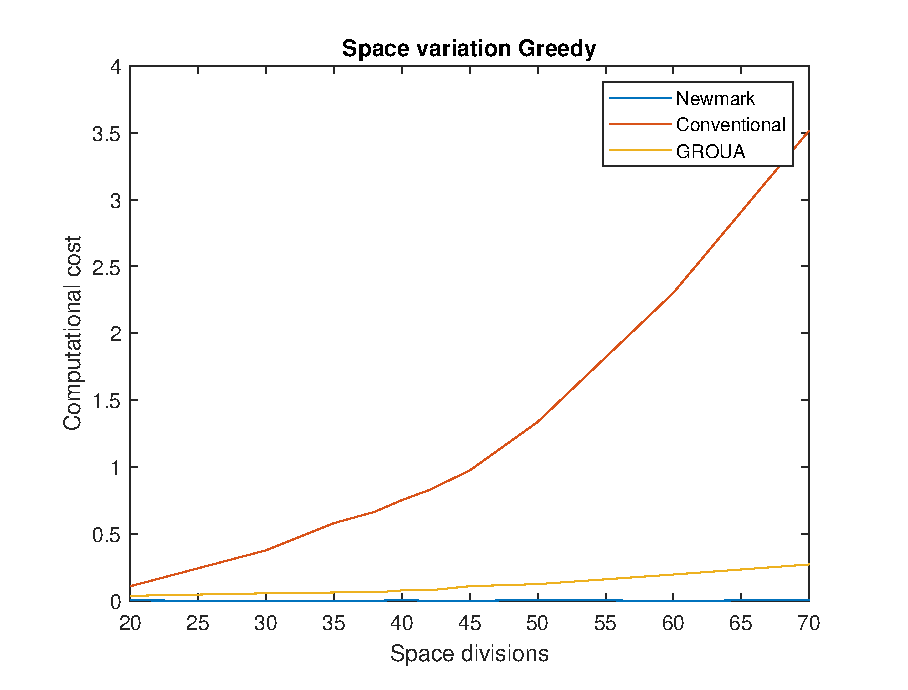
\includegraphics[width=0.75\textwidth]{CompCost3Space.eps}
\caption{Comparison between the three models} 
\label{CompCost3Space}
\end{figure}


Emphasizing the error, figure \ref{CompPropSpace} clearly shows how the order of magnitude of the error for the linear Newmark method is twice as large, which is a difference to take into account. This phenomenon is much more evident when analyzing the trend of both errors using the figure \ref{MedErrorEvoSpace}. While the error obtained using linear Newmark is clearly exponential, that obtained using GROUA is linear, even observing a peak of decline near the end.





\begin{figure}
 \centering
  \subfloat[Newmark]{
   \label{NewPropSpace}
    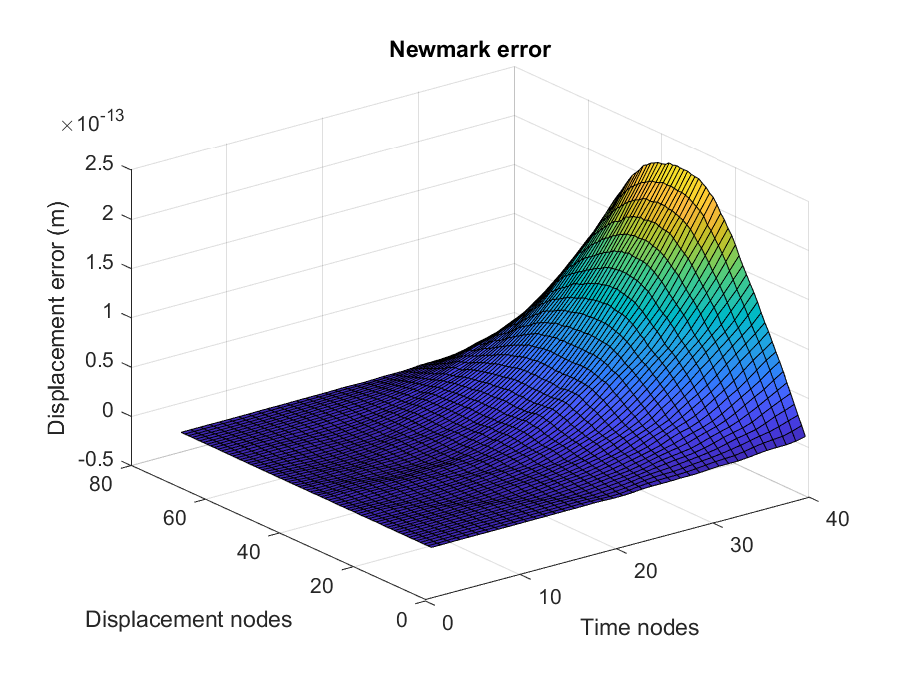
\includegraphics[width=0.5\textwidth]{NewPropErrorSpace.eps}}
  \subfloat[Greedy]{
   \label{GreedyPropSpace}
    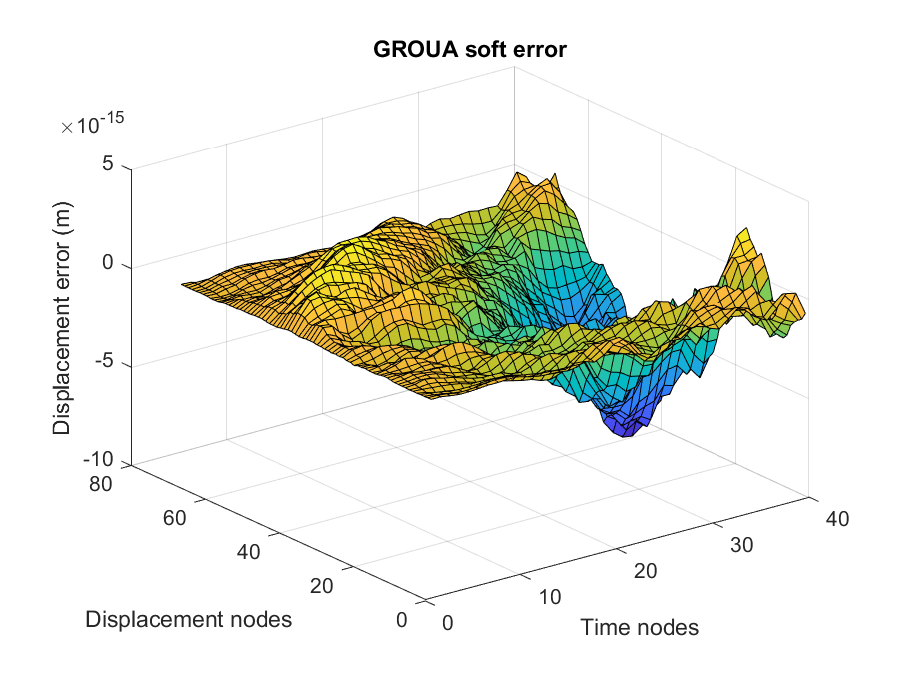
\includegraphics[width=0.5\textwidth]{GreedyPropErrorSpace.eps}}
  \caption{Comparison between Newmark and Greedy error varying the spacial discretization ($Nx=70$, $Nt=40$)}
 \label{CompPropSpace}
\end{figure}


\begin{figure}
 \centering
  \subfloat[Both]{
   \label{MedBothErrorEvoSpace}
    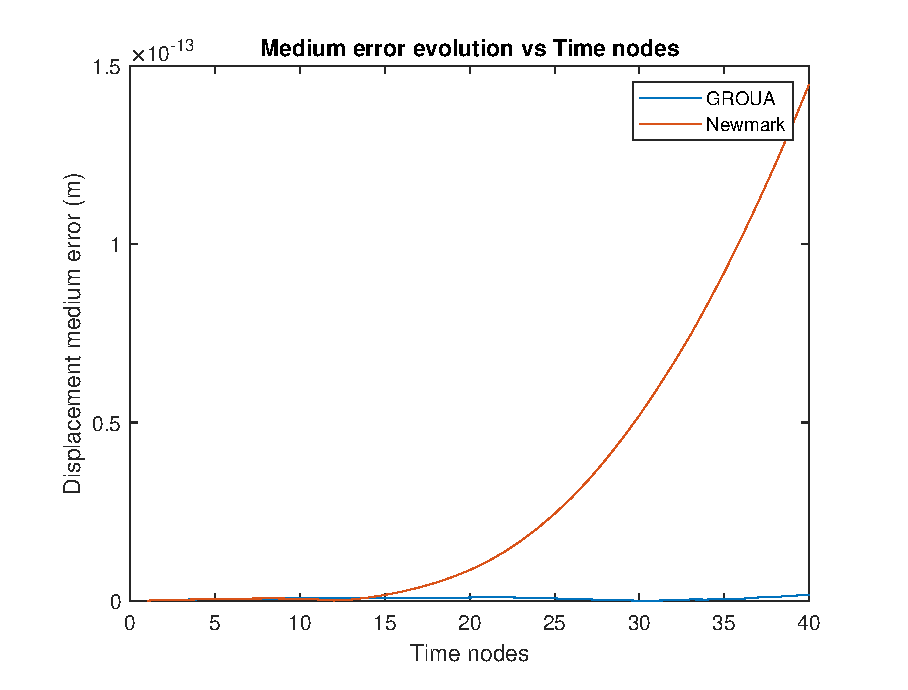
\includegraphics[width=0.5\textwidth]{MedErrorEvoSpace.eps}}
  \subfloat[Greedy]{
   \label{MedGreedyErrorEvoSpace}
    \includegraphics[width=0.5\textwidth]{MedGreedyErrorEvoSpace.eps}}
  \caption{Comparison between Newmark and Greedy medium error evolution ($Nx=20$, $Nt=70$)}
 \label{MedErrorEvoSpace}
\end{figure}



%%%  Time study  %%%

To carry out the analysis varying the time steps, the conditions and properties have been set as follows:

\begin{table}[htb]
\centering
\caption{Beam properties}
\label{tabla:propiedadesTime}
\begin{tabular}{|l|l|}
\hline
\multicolumn{2}{|c|}{Properties} \\ \hline
$m$ & $0.25$ $kg$ \\
$c$ & $0$ $N s/m$\\
$k$ & $1$ $N/m$\\
\hline
\end{tabular}
\end{table}


\begin{table}[htb]
\centering
\caption{Simulation conditions}
\label{tabla:condicionesTime}
\begin{tabular}{|l|l|}
\hline
\multicolumn{2}{|c|}{Conditions} \\ \hline
$u_0$ & $sen(\pi \tau)$ $m$ \\
$\dot{u}_0$ & $0$ $m/s$\\
$F$ & $0$ $N$\\
$f_0$ & $0$ $N$\\
$L$ & $1$ $m$\\
$T$ & $0.4$ $s$\\
$\gamma$ & $1/2$\\
$\beta$ & $1/6$ \\
$C_0$ & $80409.99$ $m$ \\
$N_x$ & $20$  \\
$N_t$ & [$20$, $30$, $35$, $38$, $40$, $42$, $45$, $50$, $60$, $70$]  \\
\hline
\end{tabular}
\end{table}

Observing the figure \ref{CompCost3Time}, as in the spatial analysis, there is a big difference between the cost when using the traditional method and the other two. The big difference with this case is that neither in the cost per linear Newmark nor in the cost per GROUA there is an upward trend for the range studied. Also, the difference between these two is even less than in the space case.


\begin{figure}
\centering
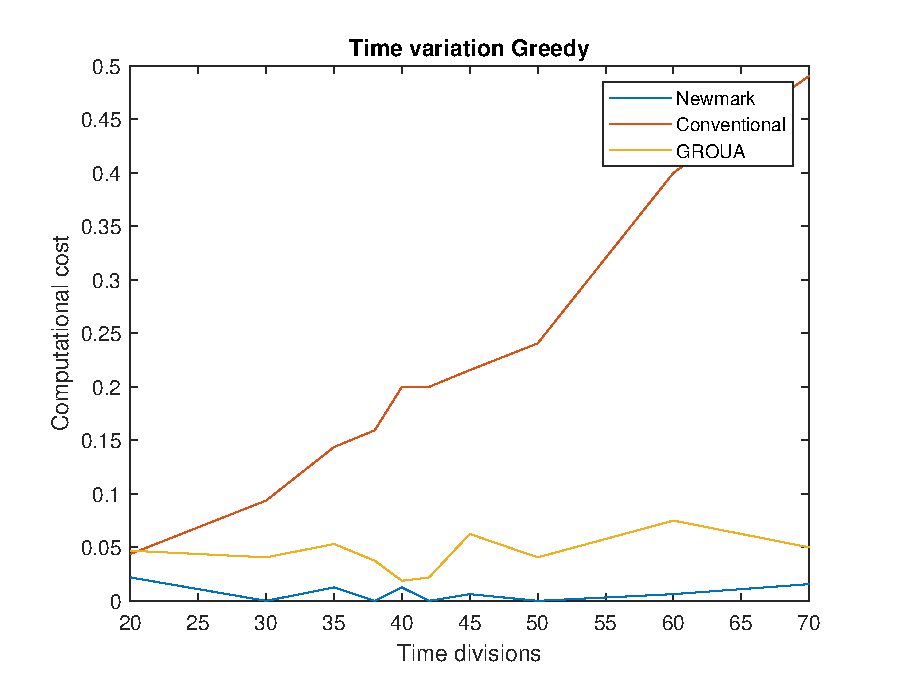
\includegraphics[width=0.75\textwidth]{CompCost3Time.eps}
\caption{Comparison between the three models ($Nx=20$, $Nt=70$)} 
\label{CompCost3Time}
\end{figure}

In the same way that it happened in the case of spatial variation, there is a difference of at least two orders of magnitude between the error for the linear Newmark method and the GROUA. As can be seen in the figure \ref{CompPropTime}, the shape is similar, although with a more exponential trend for the Newmark.
Although the most interesting result is the one obtained in the figure \ref{MedErrorEvoTime}. Figure \ref{MedBothErrorEvoTime} clearly shows the difference between the trend of both errors, but also, with figure \ref{MedGreedyErrorEvoTime} it can be concluded that the error trend when using the GROUA method is linear.



\begin{figure}
 \centering
  \subfloat[Newmark]{
   \label{NewPropTime}
    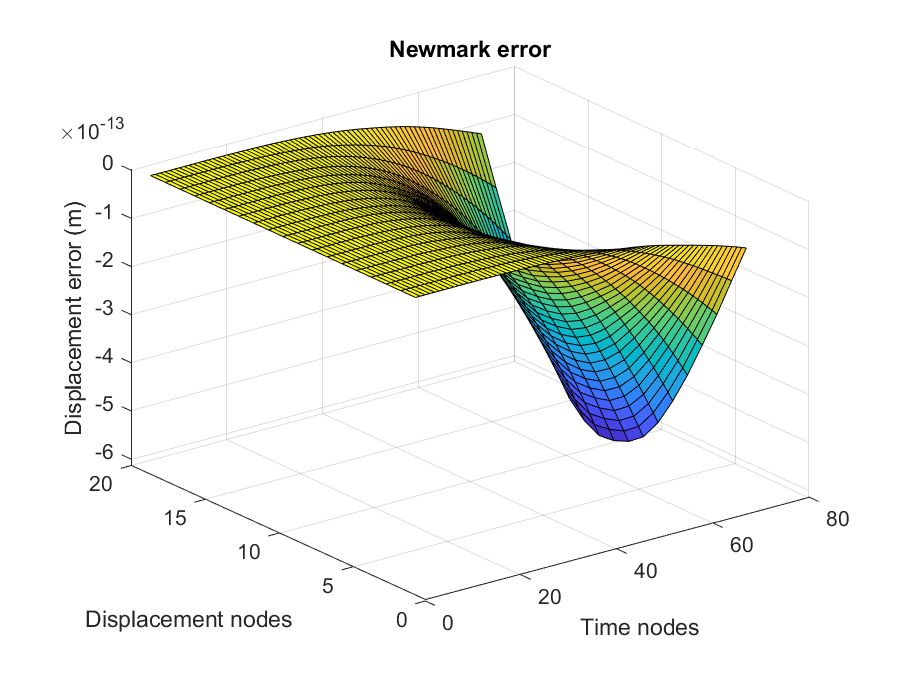
\includegraphics[width=0.5\textwidth]{NewPropErrorTime.eps}}
  \subfloat[Greedy]{
   \label{GreedyPropTime}
    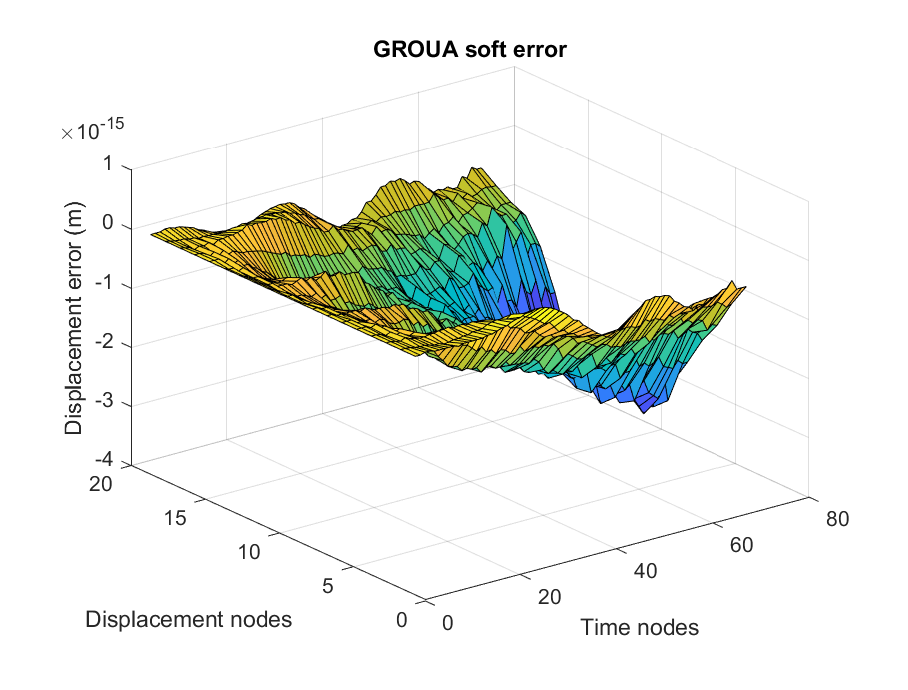
\includegraphics[width=0.5\textwidth]{GreedyPropErrorTime.eps}}
  \caption{Comparison between Newmark and Greedy error varying the temporal discretization ($Nx=20$, $Nt=70$)}
 \label{CompPropTime}
\end{figure}

\begin{figure}
 \centering
  \subfloat[Both]{
   \label{MedBothErrorEvoTime}
    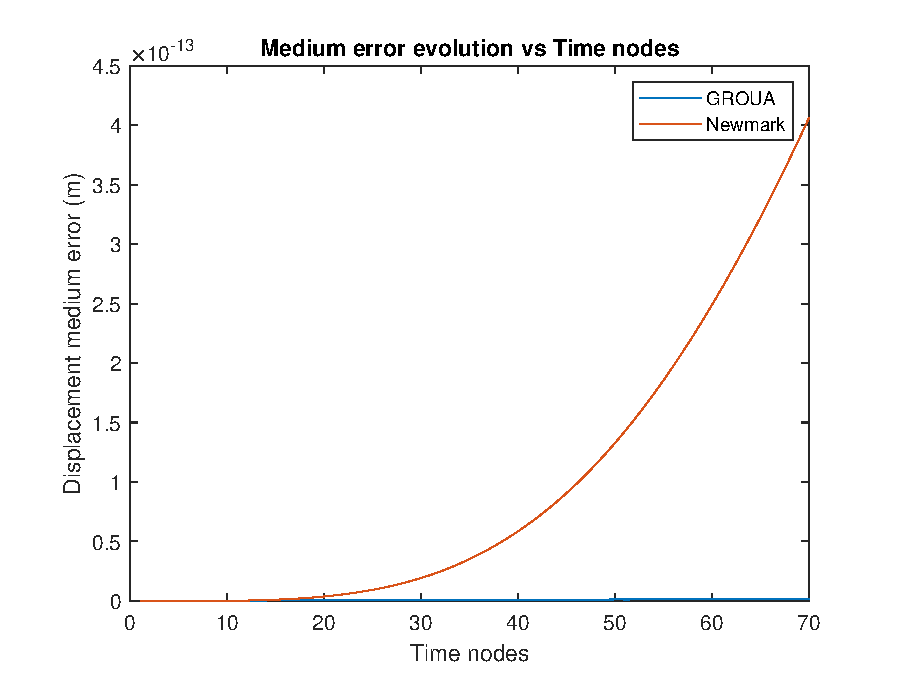
\includegraphics[width=0.5\textwidth]{MedErrorEvoTime.eps}}
  \subfloat[Greedy]{
   \label{MedGreedyErrorEvoTime}
    \includegraphics[width=0.5\textwidth]{MedGreedyErrorEvoTime.eps}}
  \caption{Comparison between Newmark and Greedy medium error evolution ($Nx=20$, $Nt=70$)}
 \label{MedErrorEvoTime}
\end{figure}





%%%%  Both study  %%%%


\subsection{A comparative study between the classical and the tensor-based Newmark's methods}

The objective of this section is to show the numerical results obtained for a specific example of the case without damping and another example with damping. These results will be compared with those obtained for the same configuration using an iterative Newmark method. The results are analyzed from three points of view, displacement, velocity and acceleration. For each of them, both the graphs are obtained along the domain for each time instant, as well as the errors between the GROUA and the Newmark method mentioned above.

\subsubsection{A comparative for an elastodynamic model without damping}

The problem treated in the example is a typical case of a beam without taking into account the damping, which is subjected to free vibration, so that no force is exerted on it. The characteristics of the beam and the conditions imposed on it are as follows:

\begin{table}[htb]
\centering
\caption{Beam properties}
\label{tabla:propiedadesNoDamping}
\begin{tabular}{|l|l|}
\hline
\multicolumn{2}{|c|}{Properties} \\ \hline
$m$ & $0.25$ $kg$ \\
$c$ & $0$ $N s/m$\\
$k$ & $1$ $N/m$\\
\hline
\end{tabular}
\end{table}


\begin{table}[htb]
\centering
\caption{Simulation conditions}
\label{tabla:condicionesNoDamping}
\begin{tabular}{|l|l|}
\hline
\multicolumn{2}{|c|}{Conditions} \\ \hline
$u_0$ & $sen(\pi \tau)$ $m$ \\
$\dot{u}_0$ & $0$ $m/s$\\
$F$ & $0$ $N$\\
$f_0$ & $0$ $N$\\
$L$ & $1$ $m$\\
$T$ & $0.4$ $s$\\
$\gamma$ & $1/2$\\
$\beta$ & $1/6$ \\
$C_0$ & $80409.99$ $m$ \\
$N_x$ & $30$  \\
$N_t$ & $20$  \\
\hline
\end{tabular}
\end{table}

As previously mentioned, the stability of the calculation has been studied, obtaining the value of the constant $C_0$ that can be seen in the table \ref{tabla:condicionesNoDamping}. Using this value, it is verified that the calculation is stable for all displacement obtained.\\

%%Imágenes desplazamiento

\begin{figure}
 \centering
  \subfloat[Displacement]{
   \label{DespVSDiv}
    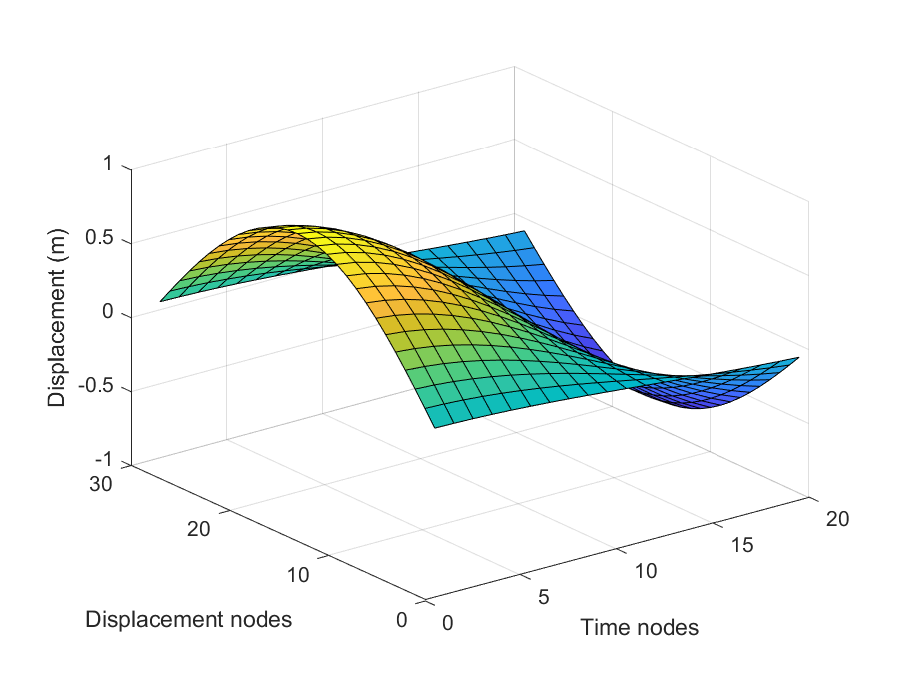
\includegraphics[width=0.5\textwidth]{DispVSDiv_Sup.eps}}
  \subfloat[Displacement error]{
   \label{DespErrVSDiv}
    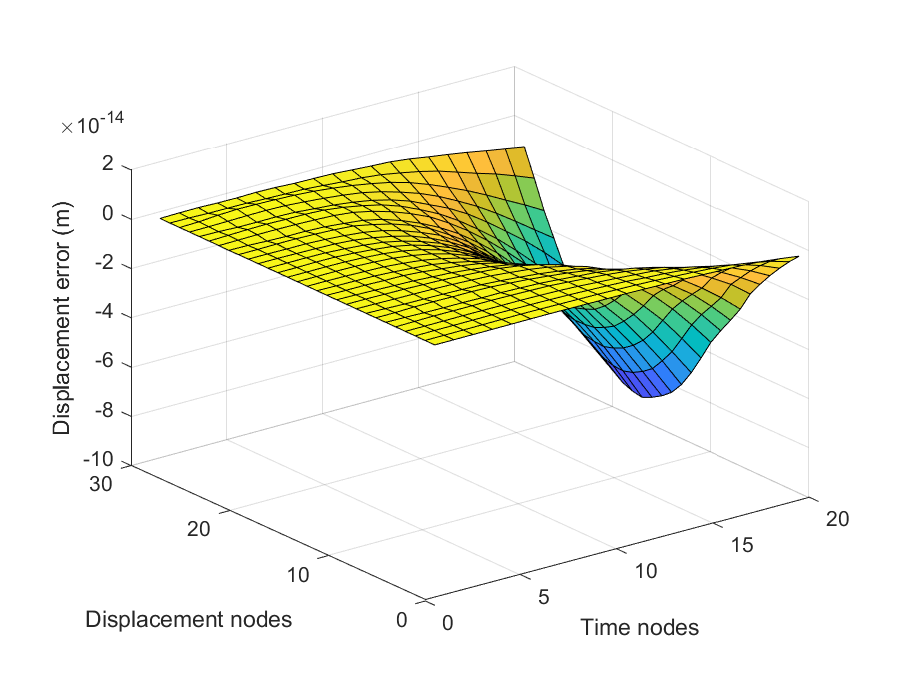
\includegraphics[width=0.5\textwidth]{DispErrVSDiv_Sup.eps}}
  \caption{Displacement and displacement error along the domain without damping}
 \label{DespVSDiv2}
\end{figure}



By imposing as an initial condition a displacement that follows a sinusoidal function, a resulting displacement is obtained like the one in the image \ref{DespVSDiv}, in which the response oscillates between a maximum and a minimum. As for the error obtained, it can be considered negligible as can be seen in the figure \ref{DespErrVSDiv}, since its order is very small compared to the values used in the problem.\\

%%Imágenes velocidad


\begin{figure}
 \centering
  \subfloat[Velocity]{
   \label{VelVSDiv}
    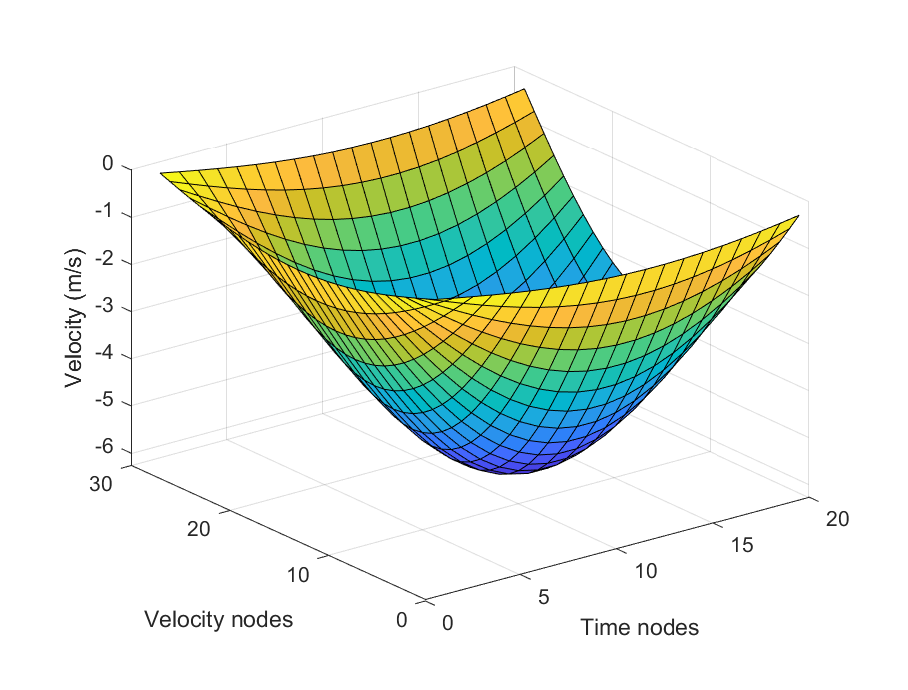
\includegraphics[width=0.5\textwidth]{VelVSDiv_Sup.eps}}
  \subfloat[Velocity error]{
   \label{VelErrVSDiv}
    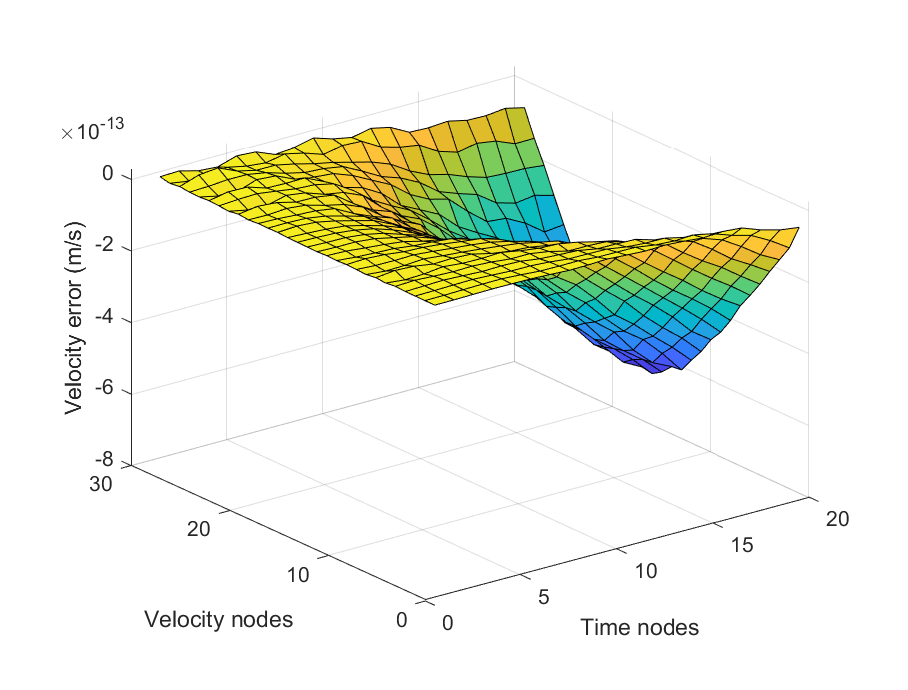
\includegraphics[width=0.5\textwidth]{VelErrVSDiv_Sup.eps}}
 \caption{Velocity and velocity error along the domain without damping}
 \label{VelVSDiv2}
\end{figure}




%%Imágenes aceleracion



\begin{figure}
 \centering
  \subfloat[Acceleration]{
   \label{AccVSDiv}
    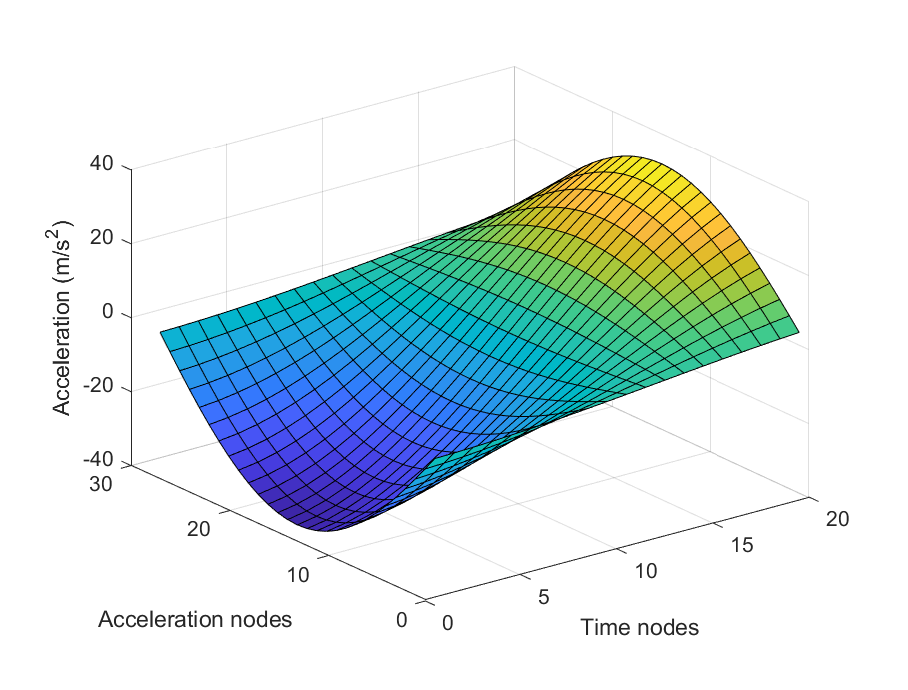
\includegraphics[width=0.5\textwidth]{AccVSDiv_Sup.eps}}
  \subfloat[Acceleration error]{
   \label{AccErrVSDiv}
    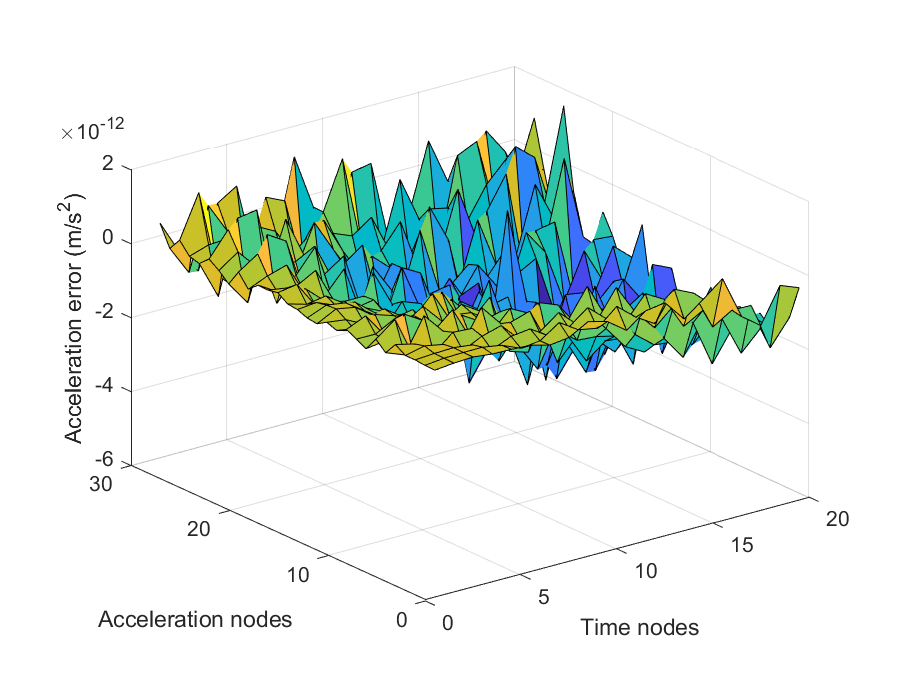
\includegraphics[width=0.5\textwidth]{AccErrVSDiv_Sup.eps}}
 \caption{Acceleration and acceleration error along the domain without damping}
 \label{AccVSDiv2}
\end{figure}



In a similar way to what happens with displacement, the graphs obtained for velocity and acceleration (figures \ref{VelVSDiv} and \ref{AccVSDiv}) are consistent. The error obtained increases by one order of magnitude for velocity and by two for acceleration, as can be seen in the figures \ref{VelErrVSDiv} and \ref{AccErrVSDiv}. Despite this, the error is essentially the same as that obtained for the displacement, since the values that are handled in the velocity and acceleration increase in the same way.\\

Something very interesting that can be observed in the figures of the errors is that said error increases with time. It is logical to think that there is an error in the GROUA due to the propagation caused by this increase. But the reality is that this error must be produced by the propagation of the linear Newmark method, since, as mentioned, it is sequential in time. To verify this phenomenon, the error between the GROUA and the traditional method has been obtained. As can be seen in the figure \ref{GreedyError}, there is no propagation of the error as the simulation time increases, which supports the hypothesis discussed above. If the figure \ref{CompGreedyNewError} is analyzed, in addition to reaffirming the non-existence of the propagation error, it is obtained that the maximum error for the sequential Newmark method is almost two orders of magnitude higher.




\begin{figure}
 \centering
  \subfloat[GROUA displacement error]{
   \label{GreedyError}
    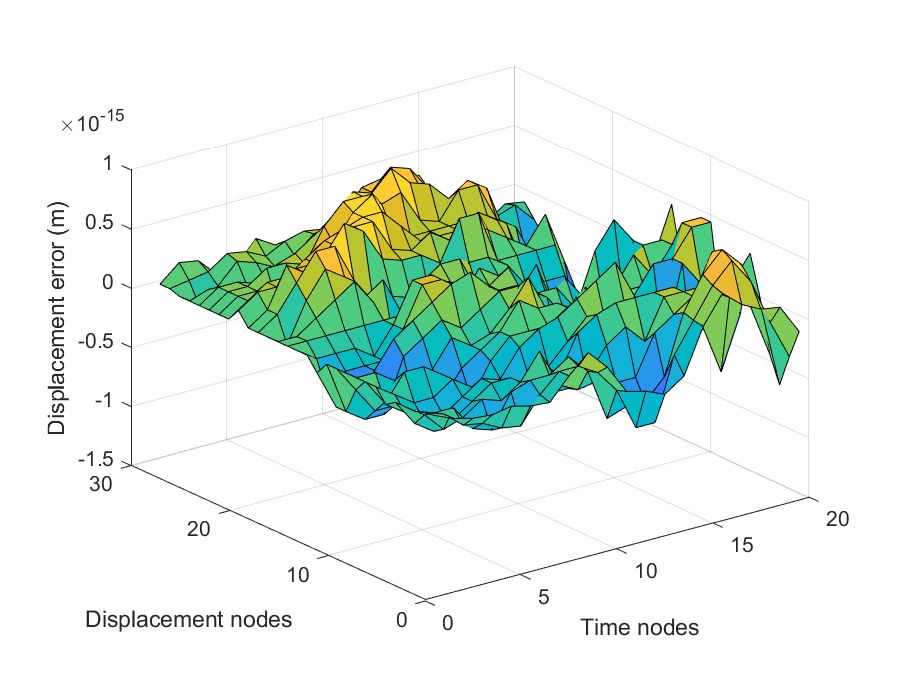
\includegraphics[width=0.5\textwidth]{DispErrVSDiv_Sup_Greedy.eps}}
  \subfloat[GROUA and Newmark displacement error]{
   \label{CompGreedyNewError}
    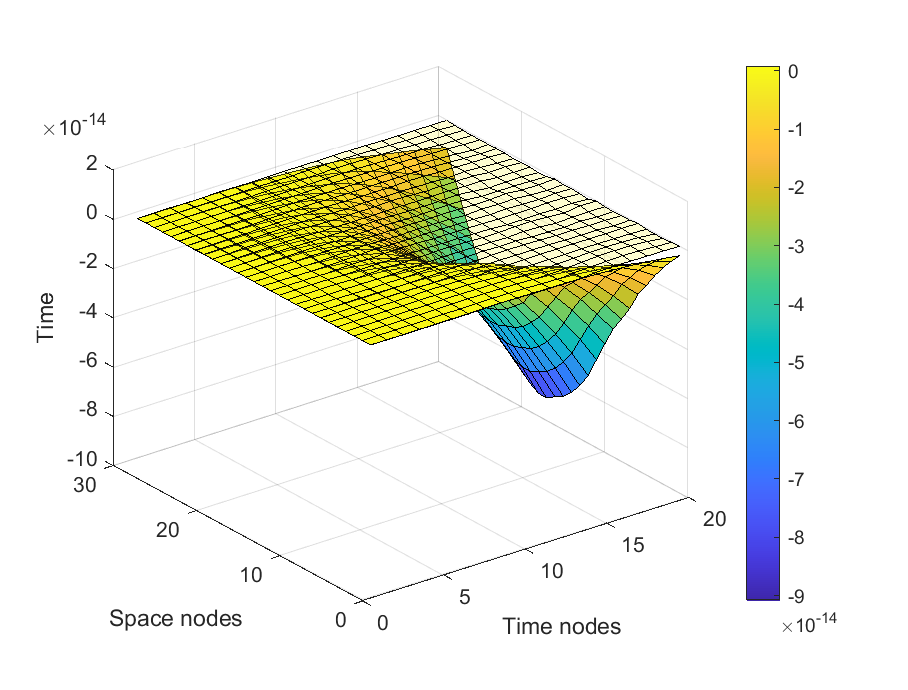
\includegraphics[width=0.5\textwidth]{DispErrVSDiv_Sup_Greedy_New.eps}}
 \caption{Propagation error analysis without damping}
 \label{PropError}
\end{figure}


As will be discussed in the conclusions, the fact that GROUA greatly improves said error may be one of the most important strengths in the use of GROUA compared to other methods that require many time steps.



\subsubsection{A comparative for an elastodynamic model with damping}


As in the previous section, the results obtained by GROUA and the iterative Newmark method will be compared, but for a case with relatively simple and two-dimensional damping. The study of a two-dimensional case is already of great interest in itself, since it could simulate a transverse load on something similar to a beam. The analysis of results is the same as the one carried out previously, being the graphs obtained and the procedure followed the same. The example deals with a beam subjected to free vibrations with the following characteristics and conditions:
 
\begin{table}[htb]
\centering
\caption{Beam properties}
\label{tabla:propiedadesD}
\begin{tabular}{|l|l|}
\hline
\multicolumn{2}{|c|}{Properties} \\ \hline
$m$ & $4$ $kg$ \\
$c$ & $1$ $N s/m$\\
$k$ & $1$ $N/m$\\
\hline
\end{tabular}
\end{table}


%%%%%%%%%%%%%%%%%%%%%%%%%%%%%%%%%
\textcolor{Red}{HAY QUE PONER LAS TABLAS BIEN}
%%%%%%%%%%%%%%%%%%%%%%%%%%%%%%%%%

\begin{table}[htb]
\centering
\caption{Beam properties and simulation conditions}
\label{tabla:propiedadesD2}
\begin{tabular}{|l|l|}
\hline
\multicolumn{2}{|c|}{Properties} \\ \hline
$m$ & $4$ $kg$ \\
$c$ & $1$ $N s/m$\\
$k$ & $1$ $N/m$\\
\hline
\end{tabular}
\begin{tabular}{|l|l|}
\hline
\multicolumn{2}{|c|}{Conditions} \\ \hline
$u_0$ &  $sen(\pi \tau)$ $m$ \\
$\dot{u}_0$ & $0$ $m/s$\\
$F$ & $0$ $N$\\
$f_0$ & $0$ $N$\\
$L$ & $1$ $m$\\
$T$ & $0.4$ $s$\\
$\gamma$ & $1/2$\\
$\beta$ & $1/6$ \\
$C_0$ & $80409.99$ \\
$N_x$ & $30$ \\
$N_t$ & $20$ \\
\hline
\end{tabular}
\end{table}

\begin{table}[ht]
\tbl{Beam properties.}
{\begin{tabular}{@{}cc@{}} \toprule
\multicolumn{2}{c}{Properties} \\
\colrule
$m$ & $4$ $kg$ \\
$c$ & $1$ $N s/m$\\
$k$ & $1$ $N/m$\\ \botrule
\end{tabular}}
\end{table}



\begin{table}[ht]
\tbl{Simulation conditions.}
{\begin{tabular}{@{}cc@{}} \toprule
\multicolumn{2}{c}{Conditions} \\
\colrule
$u_0$ &  $sen(\pi \tau)$ $m$ \\
$\dot{u}_0$ & $0$ $m/s$ \hphantom{000}\\
$F$ & $0$ $N$ \hphantom{00000}\\
$f_0$ & $0$ $N$ \hphantom{00000}\\
$L$ & $1$ $m$ \hphantom{00000}\\
$T$ & $0.4$ $s$ \hphantom{0000}\\
$\gamma$ & $1/2$ \hphantom{00000}\\
$\beta$ & $1/6$ \hphantom{00000}\\
$C_0$ & $80409.99$ \hphantom{0}\\
$N_x$ & $30$ \hphantom{000000}\\
$N_t$ & $20$ \hphantom{000000}\\ \botrule
\end{tabular}}
\begin{tabnote}
Table notes
\end{tabnote}
\begin{tabfootnote}
\tabmark{a} Table footnote A\\
\tabmark{b} Table footnote B
\end{tabfootnote}
\end{table}


As in the case without damping, using the value of $C_0$ it is obtained that the calculation is stable for all the displacements obtained. Due to the initial conditions, the same constant is obtained as in the case without damping.\\


%%Imágenes desplazamiento

By imposing the same initial conditions as before, the effect of damping can be seen clearly, as shown in figure \ref{DespVSDiv}. Compared to the case without damping, a more relaxed transition is observed over time. As main deformation, the complete bending of the beam is observed, but without changes of sign as it happened before. All this is due to the shape of the damping matrix, which is the identity matrix, and the displacement boundary condition 0.\\

As it happened in the cases without damping, the error that exists is very small compared to the displacement values that are handled. In addition, regarding the propagation error, something very similar to the case without damping happens. 


%Desplazamiento


\begin{figure}
 \centering
  \subfloat[Displacement]{
   \label{DespVSDivAmort}
    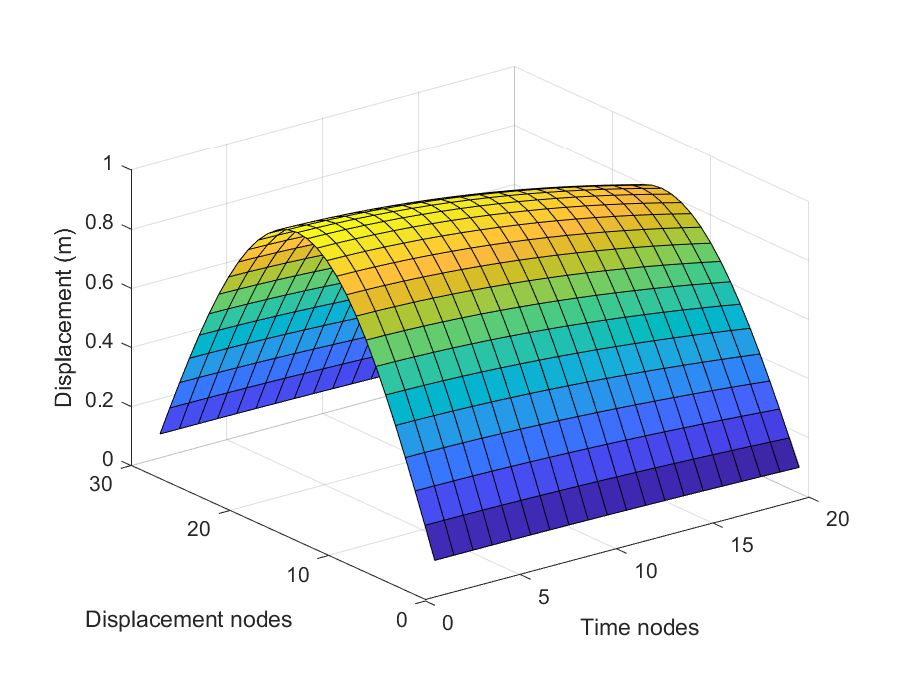
\includegraphics[width=0.5\textwidth]{DispVSDivAmort_Sup.eps}}
  \subfloat[Displacement error]{
   \label{DespErrVSDivAmort}
    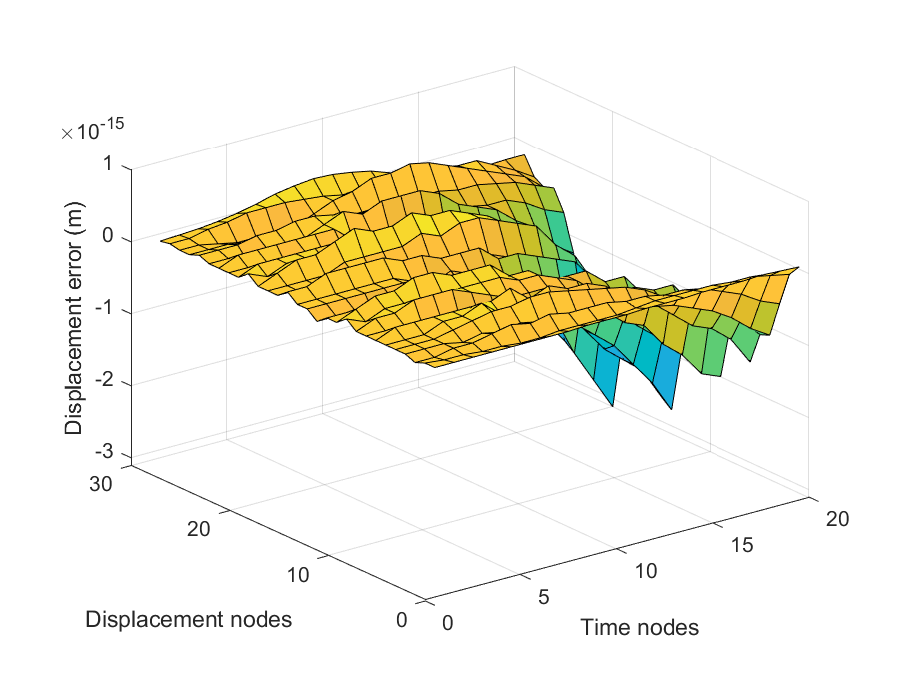
\includegraphics[width=0.5\textwidth]{DispErrVSDivAmort_Sup.eps}}
 \caption{Displacement and displacement error along the domain with damping}
 \label{DespVSDivAmort2}
\end{figure}







%Velocidad


\begin{figure}
 \centering
  \subfloat[Velocity]{
   \label{VelVSDivAmort}
    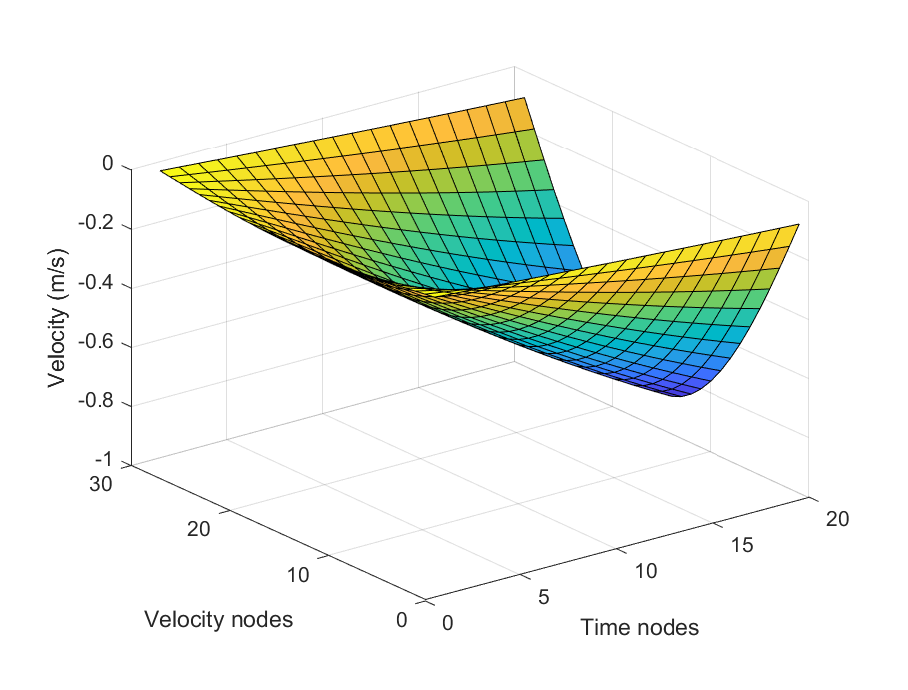
\includegraphics[width=0.5\textwidth]{VelVSDivAmort_Sup.eps}}
  \subfloat[Velocity error]{
   \label{VelErrVSDivAmort}
    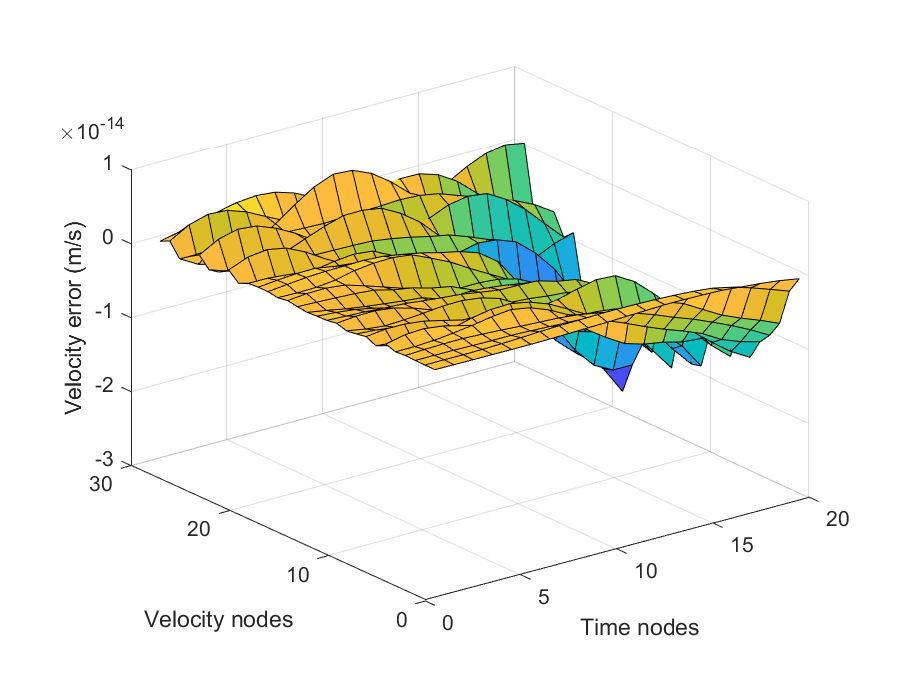
\includegraphics[width=0.5\textwidth]{VelErrVSDivAmort_Sup.eps}}
 \caption{Velocity and velocity error along the domain with damping}
 \label{VelVSDivAmort2}
\end{figure}





%Aceleracion


\begin{figure}
 \centering
  \subfloat[Acceleration]{
   \label{AccVSDivAmort}
    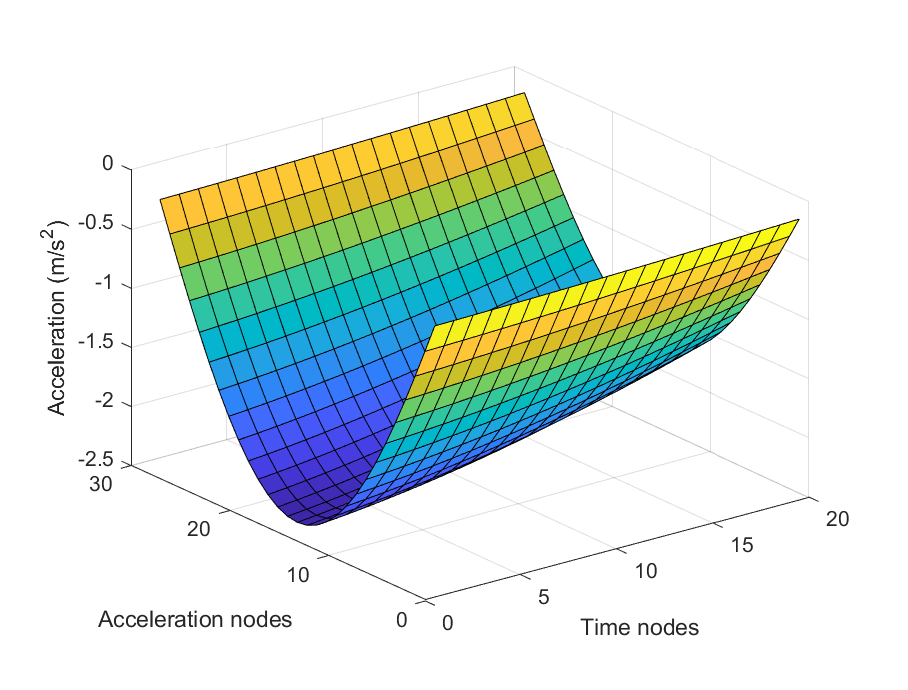
\includegraphics[width=0.5\textwidth]{AccVSDivAmort_Sup.eps}}
  \subfloat[Acceleration error]{
   \label{AccErrVSDivAmort}
    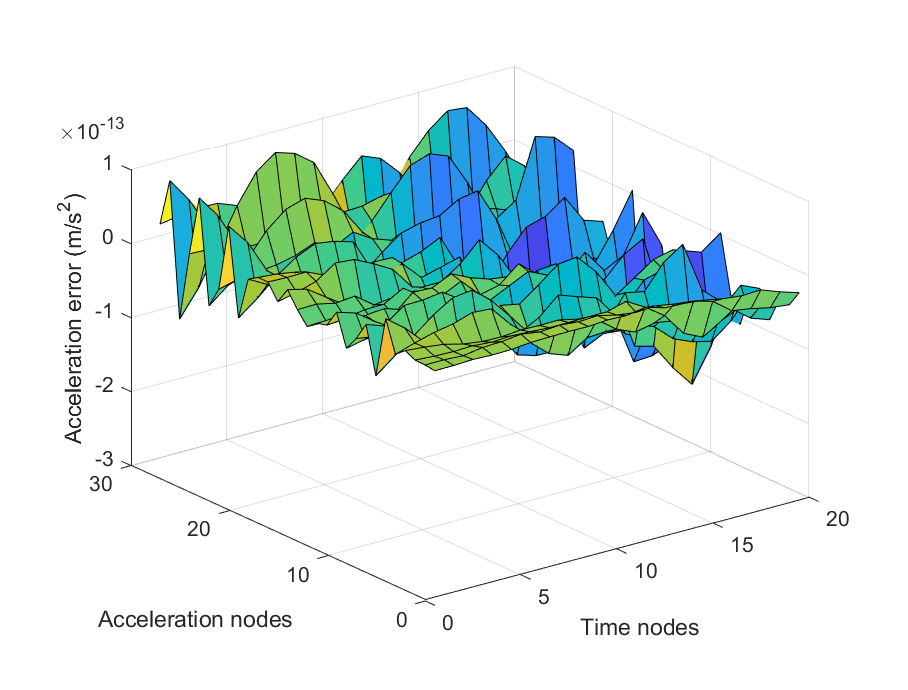
\includegraphics[width=0.5\textwidth]{AccErrVSDivAmort_Sup.eps}}
 \caption{Acceleration and acceleration error along the domain without damping}
 \label{AccVSDivAmort2}
\end{figure}

If you look at the figure \ref{GreedyErrorAmort}, you can see a slight propagation error. Despite this, specifically analyzing the figure \ref{CompGreedyNewErrorAmort}, the difference between this error and the one obtained between the GROUA and the sequential Newmark is more than one order of magnitude.
This means that, as will be discussed in the conclusions, the solution improves very significantly when using GROUA.


\begin{figure}
 \centering
  \subfloat[GROUA displacement error]{
   \label{GreedyErrorAmort}
    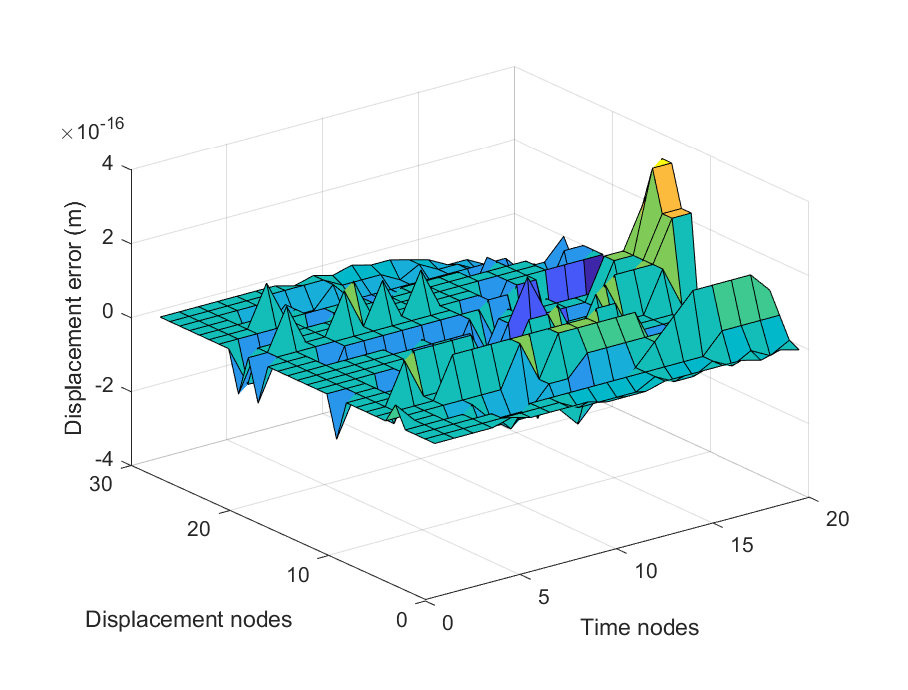
\includegraphics[width=0.5\textwidth]{DispErrVSDivAmort_Sup_Greedy.eps}}
  \subfloat[GROUA and Newmark displacement error]{
   \label{CompGreedyNewErrorAmort}
    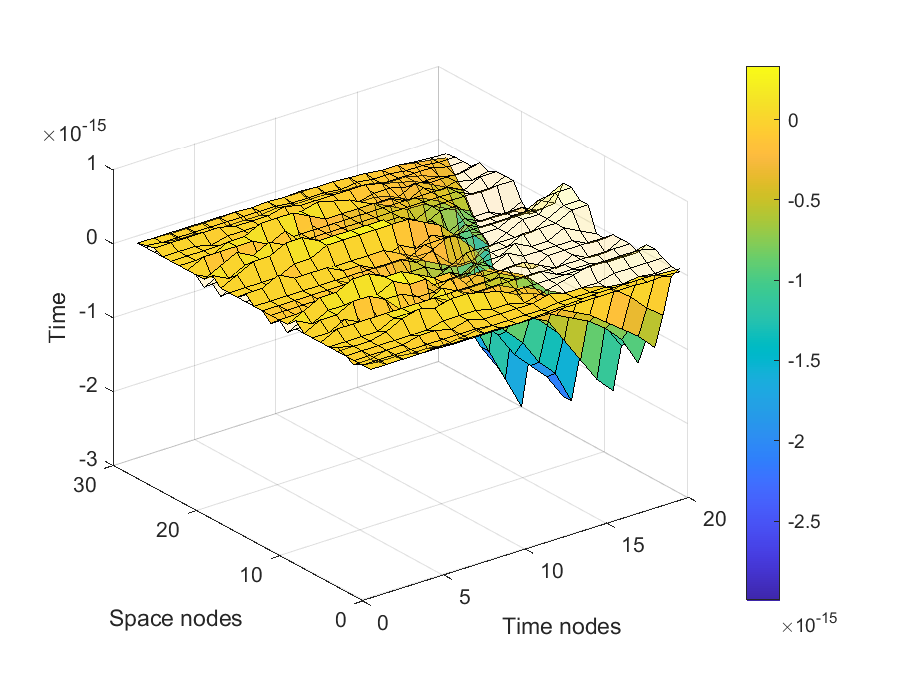
\includegraphics[width=0.5\textwidth]{DispErrVSDivAmort_Sup_Greedy_New.eps}}
 \caption{Propagation error analysis with damping}
 \label{PropErrorAmort}
\end{figure}




%%%%%%%%%%%%%%%%%%%%%%%%%%%%%%%%%%%%%%%%
%%%%%% SECCIÓN 6 %%%%%%%%%%%%%%%%%%%%%%%
%%%%%%%%%%%%%%%%%%%%%%%%%%%%%%%%%%%%%%%%


\section{Discussion and concluding remarks}

PGD-type methods are a great tool for solving problems with great costs, this has been made clear throughout the entire article. Specifically, the GROUA method used in this article solves problems posed by the elastodynamic equation faster than conventional methods, and also with great precision.

In addition to this, it is important to highlight the very basis of GROUA, since with it the entire problem is solved at once, unlike other types of methods, which are sequential. The fact of being sequential gives more fluidity and speed for cases with few elements due to its simplicity at the programming level. But precisely, due to the greater complexity, to a great treatment work on the equations involved, and above all to their tensorization, the GROUA from a certain number of elements turns out to be a much better option.\\

In addition, one of the most favorable points of the use of this type of method is the drastic reduction of the error due to propagation. The reason is obvious, the fact that the equations are solved practically in one iteration triggers this phenomenon. It must be taken into account that it cannot be said that the calculation is carried out in one iteration since, internally, the method performs several of them. But they are very few, in fact in this case studied without damping, there are three.
As has been seen in the previous section, for the study carried out, the propagation error is non-existent in the case without damping and, despite being smaller in magnitude, it is very small in the case with damping. This means that, for calculations with high simulation times, GROUA is a much better option to solve this type of problem.
As a last point to highlight, the fact that the growth trend of the error when using the GROUA method is linear is an immense advantage when calculating problems with a high computational cost. In addition to allowing more precise simulations, this phenomenon allows simulations to be carried out earlier in time without losing precision, which could be used in weather forecasting, among many other applications.

%\textcolor{Red}{Añadir menor error de propagación debido a realizar todo de una, esto se puede ver claramente en las gráficas de errores, donde conforme aumenta el tiempo aumenta el error.}\\

The reality is that using a GROUA to solve today's most complicated engineering problems can be one of the most interesting and fruitful lines of research nowadays.\\


\section*{Acknowledgment}
This section should come after the Appendices if any and should
be unnumbered. Funding information may also be included here.

\section*{References}
They are to be cited in the text in superscript
after comma and period (e.g.~word,\cite{am})
but before other punctuation marks like colons,
(e.g.~word\cite{lar}:) semi-colons and\break
question marks. If it is mentioned in the text as part of a sentence,
it should be of normal size, e.g.~see Ref.~\refcite{lar}.

\begin{thebibliography}{00}
%1
\bibitem{aiz} M. Aizenman and T. Bak, Convergence to equilibrium
in a system of reacting polymers, {\it Comm. Math. Phys.} {\bf 65}
(1979) 203--230.

%2
\bibitem{am} H. Amann, Coagulation--fragmentation
processes, {\it Arch. Rational Mech. Anal.} {\bf 151} (2000)
339--366.

%3
\bibitem{lar} L. Arlotti, A perturbation theorem for
positive contraction semigroups on $L^1$-spaces with applications to
transport equations and Kolmogorov's differential equations,
{\it Acta Appl. Math.} {\bf 23} (1991) 129--144.

%4
\bibitem{ba} L. Arlotti and J. Banasiak, Strictly substochastic
semigroups with application to conservative and
shattering solutions to fragmentation equations with mass loss,\break
{\it J. Math. Anal. Appl.} (2004), to appear.

%5
\bibitem{ge} L. Arlotti, N. Bellomo and E. De Angelis,
Generalized kinetic Boltzmann models: Mathematical structures and
applications, {\it Math. Mod. Meth. Appl. Sci.} {\bf 12} (2002)
571--596.

%6
\bibitem{ball} J. M. Ball and J. Carr, The discrete
coagulation--fragmentation equations: Existence, uniqueness and
density conservation, {\it J. Statist. Phys.} {\bf 61} (1990)
203--234.

%7
\bibitem{siak} J. Banasiak, On a diffusion-kinetic equation
arising in extended kinetic theory, {\it Math. Meth.
Appl. Sci.} {\bf 23} (2000) 1237--1256.

%8
\bibitem{jba} J. Banasiak, On an extension of Kato--Voigt
perturbation theorem for substochastic semigroups and its
applications, {\it Taiwanese J. Math.} {\bf 5}
(2001) 169--191.

%9
\bibitem{anas} J. Banasiak, On a non-uniqueness in
fragmentation models, {\it Math. Meth. Appl. Sci.}
{\bf 25} (2002) 541--556.

%10
\bibitem{boltz} J. Banasiak, On well-posedness of Boltzmann-like
semiconductor model, {\it Math. Mod. Meth. Appl. Sci.} {\bf 13}
(2003) 875--892.

%11
\bibitem{sol} J. Banasiak, Multiple solutions to linear kinetic
equations, {\it Trans. Th. Statist. Phys.} {\bf 32} (2003) 381--398.

%12
\bibitem{mcai} M. Cai, B. F. Edwards and H. Han,
Exact and asymptotic scaling solutions
for fragmentation with mass loss, {\it Phys. Rev.} {\bf A43} (1991) 656--662.

%13
\bibitem{nd} N. Dunford and J. T. Schwartz, {\it Linear Operators$,$
Part I\/$:$ General Theory} (John Wiley \& Sons, 1988).

%14
\bibitem{kje} K.-J. Engel and R. Nagel, {\it One-Parameter Semigroups
for Linear Evolution Equations}, Graduate Texts in Mathematics
(Springer-Verlag, 1999).

\end{thebibliography}

\end{document}

%%Typeout the superscript citation as:-
%%(1) word,\cite{aiz,am,lar} and word.\cite{aiz,am,lar}
%%(2) word\cite{ba}: word\cite{ba}; word\cite{ba}?
%%(3) See Ref.~\refcite{lar} --- to be cited at the text.